%%%%%%%%%%%%%%%%%%%%%%%%%%%%%%%%%%%%%%%%%
% Masters/Doctoral Thesis
%
% %%%%% IMPORTANT %%%%%
% 1) Edit Front/vars.tex
% 2) Compile Front/main.tex
% 3) Edit vars.tex
% 4) Edit precontent.tex
%
% BEFORE ANYTHING ELSE
% You can also set some interesting stuff in the preamble.tex file
% If you know what you're doing.
%%%%%%%%%%%%%%%%%%%%%%%%%%%%%%%%%%%%%%%%%

% The default font size and two-sided printing
% For a one-sided printing change the flag "twoside" to "oneside"
\documentclass[11pt, oneside, table,xcdraw]{Thesis}


%-------------------------------------------------------------------------
%   PREAMBLE AND SETTINGS
%-------------------------------------------------------------------------
% Add the preamble. You can change various settings in here
\input{preamble}

% Thesis settings. THIS IS VERY IMPORTANT YOU CHANGE
%-------------------------------------------------------------------------
% DOCUMENT VARIABLES
% NOTE: To remove links write \cmd{name} instead of \cmd[link]{name}
% NOTE: For aesthetics, at least one of these fields must be set: faculty, group
% or department
%-------------------------------------------------------------------------

% Your thesis title \ttitle
\thesistitle{System For Pratical Evaluations in Network Administration Courses}

% Your thesis type Doctoral Thesis or Masters Thesis \ttype
\thesistype{Masters Thesis}

% Your supervisor's name
\supervisor[mailto:rcprior@fc.up.pt]{Rui \textsc{Prior}}

% Your supervisor's name
% To hide the Co-Supervisor field, just comment out \cosupervisor
%\cosupervisor[mailto:name@host.com]{John \textsc{Doe}}

% Your degree name
\degree{MSc. Network and Information Systems Engineering}

% Your name
\authors[mailto:up202007895@fc.up.pt]{Diogo \textsc{Nunes}}

% Your address. Can apparently be left blank.
\addresses{}

% Your subject area
\subject{Computer Science}

% Keywords for your thesis
\keywords{Proxmox VE, GNS3, automation, Nornir, FastAPI, asynchronous, communication, emulation, teaching tool}



% Your university's name
\university{Universidade do Porto}
% Your university's name in capitals
\UNIVERSITY{UNIVERSIDADE DO PORTO}

% Your faculty's name
% To hide the Faculty field, just comment out \FACULTY and \Faculty
\faculty{Faculty of Sciences of the University of Porto}
% Your faculty's name in capitals
\FACULTY{FACULTY OF SCIENCES OF THE UNIVERSITY OF PORTO}

% Your department's name
% To hide the Department field, just comment out \DEPARTMENT and \department
\department{Department of Computer Science}
% Your department's name in capitals
\DEPARTMENT{DEPARTMENT OF COMPUTER SCIENCE}

% Your research group's name
% To hide the Group field, just comment out \GROUP and \group
%\group[http://www.groupurl.com]{Research Group}
% Your research group's name in capitals
%GROUP[http://www.groupurl.com]{RESEARCH GROUP}

% ------------------


%-------------------------------------------------------------------------
%	DOCUMENT
%-------------------------------------------------------------------------

\begin{document}

% Start counting pages in an unused scheme to fix backref
\pagenumbering{Alph}

% Includes the front pages (cover and etc.)
\pagestyle{empty}
\includepdf[pages={1},pagecommand={},scale=1]{Front/main}
\cleardoublepage
\includepdf[pages={2},pagecommand={},scale=1]{Front/main}
\cleardoublepage
\pagestyle{fancy}

%----------- Failed attempt to make cover page in latex ------------------

% Cover page
%\newgeometry{bindingoffset=0cm,
%	top=1.27cm,
%	outer=1.27cm,
%	inner=1.27cm,
%	bottom=1.27cm}

%\pagestyle{empty}
%
%\begin{picture}(-5,0)(2.5,0)
%% MSc symbol
%\put(331.8,-808.061){\includegraphics[width=267.6pt,height=464.25pt]{Front/Cover/MSc.png}}
%% FEUP logo
%\put(382,-345){\includegraphics[width=155.9pt]{Front/Cover/FEUP.png}}
%% FCUP logo
%\put(360.5,-293){\includegraphics[width=183pt]{Front/logos/fcup.png}}
%\end{picture}
%
%%\makebox[12cm][l]{\ttitle}
%
%\vfill
%\parbox[t][12cm][t]{12cm}{\bf\fontsize{55}{0}\selectfont\ttitle}
%\vfill
%
%\restoregeometry

%-------------------------------------------------------------------------

% Use roman page numbering style (i, ii, iii, iv...) for the pre-content pages
\frontmatter

% Title page
%\maketitle

% Edit this file!

%-------------------------------------------------------------------------
%	QUOTATION PAGE
%-------------------------------------------------------------------------
%\quotepage{Matt Smith as \emph{The Doctor}, written by Matthew Graham}
%{
%	I am and always will be the optimist, the hoper of far-flung hopes and the
%	dreamer of \newline improbable dreams
%}

%-------------------------------------------------------------------------
%	DEDICATORY
%-------------------------------------------------------------------------

%\begin{dedicatory}
%	Dedicated to (optional) 
%\end{dedicatory}

%-------------------------------------------------------------------------
%	ACKNOWLEDGEMENTS PAGE
%-------------------------------------------------------------------------
\addtocontents{toc}{\protect\setcounter{tocdepth}{-1}}
\begin{acknowledgements}

Firstly i would like to thank my friends and family for encouraging me to pursue both my Bachelor's and Master's degrees. 
Their love and support were fundamental in this endeavor.

Additionally i want to express my sincerest gratitude to my girlfriend Daniela for all the love, support, company, all 
the time spent playing board games and just being herself, as well as her family for all the support that they give me.

Furthermore i would like to thank my Master's supervisor Professor Rui Prior for allowing me to explore this topic, as well 
as all the ideas and feedback he gave me during development.

Likewise i would like to thank Instituto de Telecomunicações (UIDB/50008/2020) for hosting this work.

Lastly i would like to thank Ginjas, for just being him.

Thank you.

\vspace*{10cm}
\newfontfamily\sinhalaFont{Noto Sans Sinhala}
\tikz[baseline]{
  \node[opacity=0.05, text=black, font=\sinhalaFont] at (0,0) {ඞ};
}

\end{acknowledgements}
\addtocontents{toc}{\protect\setcounter{tocdepth}{3}}
%\addvspacetoc{0.3cm} % Add a gap in the Contents, for aesthetics


%-------------------------------------------------------------------------
%	ABSTRACT PAGE (PORTUGUESE)
%-------------------------------------------------------------------------
\addtocontents{toc}{\protect\setcounter{tocdepth}{-1}}
\begin{abstract}[
	thesistitle={Sistema para Avaliações Práticas de Administração de Redes },
	title={Resumo},
	degree={Mestrado em Engenharia de Redes e Sistemas Informáticos},
	nameconnector={por},
        keywordsname={Palavras-chave},
        keywords={ Proxmox VE, GNS3, automação, Nornir, FastAPI, assíncrono, comunicação, emulação, ferramenta de ensino}]
\begin{otherlanguage}{portuguese}

Os métodos convencionais de formação em rede de computadores, que dependem fortemente do hardware físico, são muitas vezes proibitivamente 
caros e não são escaláveis. As tecnologias de virtualização e emulação resolvem esta limitação, permitindo a execução 
simultânea de vários dispositivos simulados numa única máquina. No entanto, a avaliação da correção das configurações dos 
dispositivos de rede continua a ser um processo manual, propenso a erros, em que configurações incorrectas podem conduzir 
a falhas críticas em toda a rede.

A primeira fase deste projeto, conduzida por um estudante anterior, centrou-se na investigação da viabilidade de construir um sistema deste 
tipo e na produção de um conjunto de componentes soltos. Este trabalho representa a segunda fase, focando-se no desenho e implementação de um 
sistema para avaliação automática de topologias de rede, com suporte para um ambiente de dispositivos heterogéneos, no seguimento direto de um 
trabalho anterior. O sistema terá como objetivo fornecer um ambiente de trabalho completo para os alunos, uma interface Web para que tanto os 
alunos como os professores possam interagir com a plataforma e capacidades para automatizar a avaliação das configurações feitas pelos 
alunos, permitindo que os professores se concentrem no ensino e na orientação dos alunos, em vez de terem de efetuar 
verificações manuais repetitivas dos trabalhos dos alunos.

Os desenvolvimentos deste projeto incluem a extensão e integração do trabalho anterior, bem como o desenvolvimento de uma 
aplicação web utilizando FastAPI para alavancar as capacidades de comunicação assíncrona que se revelaram essenciais para 
garantir que o sistema pode escalar.


\end{otherlanguage}
\end{abstract}
\addtocontents{toc}{\protect\setcounter{tocdepth}{3}}
%-------------------------------------------------------------------------
%	ABSTRACT PAGE
%-------------------------------------------------------------------------
\addtocontents{toc}{\protect\setcounter{tocdepth}{-1}}
\begin{abstract} 

Conventional computer network teaching methods, which depend heavily on physical hardware, are often prohibitively expensive and lack scalability. 
Virtualization and emulation technologies address this limitation by allowing multiple simulated devices to run concurrently 
on a single system. Nevertheless, assessing the correctness of network device configurations continues to be a manual, 
error-prone process, where misconfigurations can lead to critical failures across the network.

The first phase of this project, conducted by a previous student, focused on investigating the viability of building such a system and 
producing a set of loose components. This work represents the second phase,centered on designing and implementing a system for automated assessment 
of network topologies, designed to support a diverse range of network devices. Building upon previous research, the system aims to deliver a complete, 
web-based working environment where both students and instructors can interact with the platform. Its key feature is the automation of configuration 
assessments made by students, which reduces the manual workload for instructors, allowing them to focus more on teaching and guiding 
rather than repetitive checking of assignments.

The developments of this project include the extension and integration of previous work as well as the development of a web 
application using FastAPI to leverage asynchronous communication capabilities which proved essential to ensure the system can 
scale.


\end{abstract}
\addtocontents{toc}{\protect\setcounter{tocdepth}{3}}

%-------------------------------------------------------------------------
%	LIST OF CONTENTS/FIGURES/TABLES
%-------------------------------------------------------------------------

\addtocontents{toc}{\protect\setcounter{tocdepth}{-1}}

\tableofcontents % Write out the Table of Contents

\addtocontents{toc}{\protect\setcounter{tocdepth}{3}}
\addvspacetoc{0.3cm}

%\listoftables % Write out the List of Tables

\listoffigures % Write out the List of Figures



%\addvspacetoc{0.3cm}

%-------------------------------------------------------------------------
%	PHYSICAL CONSTANTS/OTHER DEFINITIONS
%-------------------------------------------------------------------------

%\begin{listofcontants}
%	\const{My little ponny test of magical rainbow}{$mn/mp$}
%    {$2.997\ 924\ 58\times10^{8}\ \mbox{ms}^{-\mbox{s}}$}
%   \const{Vaccuum permeability test of magical rainbow for a specific case of
%   condensed matter physics}
%   {$\epsilon_0$}{$2.997\ 924\ 58\times10^{8}\ \mbox{ms}^{-\mbox{s}}$}
%	\const{Speed of Light test of magical rainbow}{$c$}
%    {$2.997\ 924\ 58\times10^{8}\ \mbox{ms}^{-\mbox{s}}$}
%\end{listofcontants}


%-------------------------------------------------------------------------
%	SYMBOLS
%-------------------------------------------------------------------------

%\begin{listofsymbols}
%	\symb{$F_{\mu\nu}$}{Maxwell tensor}{F}
%	\symb{$a$}{distance}{m}
%	\\
%	\symb{$\omega$}{angular frequency}{rads$^{-1}$}
%\end{listofsymbols}


%-------------------------------------------------------------------------
%	NOTATION
%-------------------------------------------------------------------------

% \newcommand\notationname{Notation and Conventions}
% \addtotoc{\notationname}
% \fancyhead[LO]{\textsc{\notationname}}

% \input{Notation}



%-------------------------------------------------------------------------
%	ABBREVIATIONS
%-------------------------------------------------------------------------

\newacronym{cs}{CS}{Computer Science}

\newacronym{dcc}{DCC}{FCUP-Department of Computer Science}

\newacronym{gns3}{GNS3}{Graphical Network Simulator-3}

\newacronym{rest}{REST}{Representational State Transfer}

\newacronym{api}{API}{Application Programming Interface}

\newacronym{qemu}{QEMU}{Quick Emulator}

\newacronym{iou}{IOU}{IOS on Unix}

\newacronym{ios}{IOS}{Internetworking Operating System}

\newacronym{vpcs}{VPCS}{Virtual PC Simulator}

\newacronym{vm}{VM}{Virtual Machine}

\newacronym{http}{HTTP}{Hypertext Transfer Protocol}

\newacronym{json}{JSON}{JavaScript Object Notation}

\newacronym{wsgi}{WSGI}{Web Server Gateway Interface}

\newacronym{asgi}{ASGI}{Asynchronous Server Gateway Interface}

\newacronym{oas}{OAS}{OpenAPI Specification}

\newacronym{pve}{Proxmox VE}{Proxmox Virtual Environment}

\newacronym{kvm}{KVM}{Kernel-based Virtual Machine}

\newacronym{lxc}{LXC}{Linux Containers}

\newacronym{jwt}{JWT}{JSON Web Token}

\newacronym{ldap}{LDAP}{Lightweight Directory Access Protocol}

\newacronym{ssh}{SSH}{Secure Shell}

\newacronym{lvm}{LVM}{Logical Volume Manager}

\newacronym{lvmt}{LVM-Thin}{LVM Thin Provisioning}

\newacronym{cow}{CoW}{Copy-on-Write}

\newacronym{orm}{ORM}{Object-Relational Mapping}

\newacronym{spice}{SPICE}{Simple Protocol for Independent Computing Environments}

\newacronym{dry}{DRY}{Don't Repeat Yourself}

\newacronym{uuid}{UUID}{Universally Unique Identifier}

\newacronym{ui}{UI}{User Interface}

\newacronym{gui}{GUI}{Graphical User Interface}

\newacronym{cpu}{CPU}{Central Processing Unit}

\newacronym{virl}{VIRL}{Virtual Internet Routing Lab}

\newacronym{vnc}{VNC}{Virtual Network Computing}

\newacronym{yaml}{YAML}{YAML Ain't Markup Language}

\newacronym{ssd}{SSD}{Solid State Drive}



\printglossary[type=\acronymtype,title={List of Abbreviations}]



%-------------------------------------------------------------------------
%	THESIS CONTENT - CHAPTERS
%-------------------------------------------------------------------------

\addvspacetoc{0.3cm}

% Begin numeric (1,2,3...) page numbering
\mainmatter

\pagestyle{fancy}
\renewcommand{\chaptermark}[1]{\markboth{\thechapter. \textsc{#1}}{}}
%\fancyhead[LO]{\leftmark}


%%% -----------  ADD CHAPTERS HERE ------------------ %%%

% Chapter Template

% Main chapter title
%\chapter[toc version]{doc version}
\chapter{Introduction}

% Short version of the title for the header
%\chaptermark{version for header}

% Chapter Label
% For referencing this chapter elsewhere, use \ref{ChapterTemplate}
\label{Chapter1Introduction}

% Write text in here
% Use \subsection and \subsubsection to organize text

Network administration remains a fundamental discipline within\ac{cs}, given the central role that networked systems play in the functioning, 
scalability, and security of modern digital infrastructures.

Modern organizations require professionals who can design, configure, and troubleshoot increasingly complex network environments. 
Effective education must therefore bridge theoretical knowledge with practical implementation, particularly through hands-on learning 
that simulates real-world scenarios. Yet current training and assessment methods fail to meet these needs at scale, creating a growing gap 
between academic preparation and professional requirements.

This project aims to build an initial version of a system capable of assisting training in the topic of network administration, building upon previous 
work of \citet{santos2024} which solved a series of individual problems relevant to this topic, without building a system out of them.

\section{Need for Automated Assessment}

  Practical assessments are essential to prepare students for real-world challenges, enabling them to apply 
  theoretical knowledge and develop hands-on skills. However, traditional assessment methods face significant limitations.

  Creating a physical network environment for practical assessments is sure to be costly and challenging to scale for 
  large student populations. 
  While emulation and virtualization technologies offer cost-effective alternatives for creating flexible practice environments, 
  they lack built-in automated assessment capabilities. 
  Instructors must manually review each students' network assignment configuration—a process that is:

  \begin{itemize}
    \item \textbf{Time-consuming}: Manual checks grow linearly with class size.
    \item \textbf{Error-prone}: Human reviewers may overlook misconfigurations.
    \item \textbf{Risk of inconsistency}: Automated assessment ensures fully deterministic and consistent evaluation.
  \end{itemize}

  Automating assessments would reduce instructor workload, freeing time for student support as well as ensure consistent, objective grading 
  and simultaneously enable immediate feedback for learners.

  Previous work by \citet{santos2024} has shown that it is possible to automate the validation of basic network commands, such as verifying 
  the output of a ping command between a specific machine and a target IP address. This demonstrates that connectivity checks 
  can be automated, paving the way for network automated assessment.

  \subsection{Limitations of Current Solutions}

    Existing approaches to network education suffer from two critical gaps:

    \begin{enumerate}
        \item \textbf{Single-vendor focus}: Most tools (e.g., Cisco's Packet Tracer) are designed for specific vendor ecosystems, failing 
        to prepare students for heterogeneous real-world networks where multi-vendor interoperability is essential.
        \item \textbf{Missing assessment component}: Some education institutions' curricula, such as our case in\ac{dcc}, forgo practical 
        assessments entirely, meaning students complete networking exercises without getting feedback or validation. This lack of feedback 
        can lead to students having gaps in their knowledge, hindering their performance when they join the workforce, as they may not have 
        acquired sufficient practical skills in the identification and solving of common problems.
    \end{enumerate}

\section{Aims and Objectives}

  Designing and implementing a system that can automatically evaluate network administration assignments is one of the aims 
  of this work. It will be utilised as a tool in classes and tests, allowing instructors to spend more time directly helping 
  and guiding students.

  One of the objectives needed to accomplish this, is to have such a system be able to perform assessments whenever requested 
  by a student, in a fully automated manner.
  To have a wide range of support for vendors and device types is also highly desirable as exposing students to as much 
  variety as possible will better prepare them for more heterogeneous environments of the real world.
  It will also be important to have assessment for configurations as well as connectivity.

  Another aim of this project is to create a modular and cohesive back-end system out of the components created by 
  \citet{santos2024}.
  Achieving this will require further development of the components as well as creating capabilities to communicate between 
  them.

  

\section{Organization}

  Besides the Introduction, this work includes 6 more chapters:

  \begin{enumerate}
      \item \textbf{Chapter 2} presents an overview of the system components and underlying technologies.
      \item \textbf{Chapter 3} reviews related work, highlighting lessons learned and how this project differentiates itself from existing solutions.
      \item \textbf{Chapter 4} provides a detailed description of the system architecture and its layers. It also outlines the project's functional use cases.
      \item \textbf{Chapter 5} focuses on implementation details, emphasizing design decisions and their realization.
      \item \textbf{Chapter 6} discusses performance evaluation results, demonstrating the scalability of solutions introduced in this work.
      \item \textbf{Chapter 7} gives an overview of met aims and objectives, reviews lessons learned throughout, and goes 
      over ideas for future work.
  \end{enumerate}
% Chapter Template

% Main chapter title
%\chapter[toc version]{doc version}
\chapter{Background}

% Short version of the title for the header
%\chaptermark{version for header}

% Chapter Label
% For referencing this chapter elsewhere, use \ref{ChapterTemplate}
\label{Chapter2Background}

% Write text in here
% Use \subsection and \subsubsection to organize text

This chapter lays the technical groundwork for our project, with the aim to provide the reader with the necessary background to 
understand the context and technical foundations of this project. The goal of the system is to automatically evaluate network 
assignments by validating configurations and executing tests across various devices within a virtual network. Achieving this 
will require the coordination of several components and services in order to support an automated solution capable of providing 
each student with a correctly provisioned environment. 

While a more detailed architecture will be presented in Chapter~\ref{Chapter4SystemArchitectureDesign}, here we will introduce the 
concepts and technologies that make this project possible. These include virtualization technologies to host students' work environments 
as well as the network devices in them, technologies that support our orchestration needs, web frameworks for user interaction and asynchronous 
technologies to enhance scalability.

\section{Virtualization}
  Virtualization is the process of creating a virtual version of physical resources, such as routers, switches, or even
  entire computers. In the context of this project, it is used to create\ac{vm}s to provide students with a 
  work environment consisting of a virtual network, itself comprised of various types of virtualized devices. This approach 
  enhances scalability and reduces costs, as it allows multiple\ac{vm}s to be run on a single physical machine.

  In our project we will utilize \textbf{emulation} and \textbf{simulation}. 

  \begin{itemize}
    \item \textbf{Emulation} is the process of replicating the exact behavior of a hardware or software system in a virtual environment, 
    reproducing even its bugs and limitations. This is useful for various things like testing software on different platforms, 
    running legacy software on modern hardware and even running potentially harmful software in a safe isolated environment.
    Emulation will be used wherever possible to provide students with a work environment that resembled the real world as much as 
    possible to best develop their network skills.
    \item \textbf{Simulation} models aspects of the behaviour of a device, without replicating the underlying hardware or software.
    This results in a simpler, less resource intensive model, though it may not fully capture the real devices' behavior.
    Simulation will be used to simulate the behaviour of certain, simpler and generic, network devices and PCs.
  \end{itemize}

  This project relies on both, as they enable the use of the the devices in the virtual work environments students will use to 
  complete their assignments. These environments are hosted within\ac{vm}s that run on a virtualization platform. These will be 
  discussed in further detail, in Section~\ref{sec:chap2_gns3} and Section~\ref{sec:chap2_pve}.

  \subsection{Virtualized Work Environments}
    Creating a physical lab for students to learn and practice networking skills can be labor and time intensive as well as costly for larger student populations.
    To tackle this challenge we devised virtualized work environments wth existing tools and technologies, where a student can interact with a unique instance of a 
    virtualized network, consisting of multiple devices. Then, by virtualizing these work environments, we can 
    host several instances simultaneously over a single physical machine, increasing the number of students supported without an increase of hardware 
    requirements.
    
    This approach offers significant benefits over physical lab infrastructures:

    \begin{itemize}
      \item \textbf{Resource Efficiency}: Single physical host can support multiple concurrent student environments, each with multiple devices.
      \item \textbf{Operational Characteristics}:
      \begin{itemize}
          \item Fast environment provisioning through template\ac{vm}s.
          \item Possibility of state preservation via\ac{pve}'s snapshot/restore functionality.
          \item Support for diverse operating systems through virtualization technologies.
      \end{itemize}
    \end{itemize}

    The combined use of\ac{pve} as a virtualization platform and\ac{gns3} for network emulation presents a flexible and cost-effective solution 
    for scalable networking education.


\section{GNS3}
\label{sec:chap2_gns3}
  \ac{gns3} is an open-source graphical network emulator software that allows the user to create complex network topologies 
  and interact with the various devices in it. It is widely used for educational purposes and is often used in preparation 
  for professional network certifications like the Cisco Certified Network Associate (CCNA).

  \ac{gns3} employs a simple drag and drop interface to allow users to add new devices, make links between them 
  and even add textual annotations. The software allows users to interact with the devices by way of a console or even a\ac{gui}
  if the device supports it. It also allows users to export their topologies to be shared with others, which can
  be useful for teachers to provide students with a pre-configured assignment to work on.

  Additionally, there is support for packet capturing, which is essential for students to develop their debugging and 
  troubleshoting skills. Finally, it can also be interacted with via a \ac{rest}\ac{api}, which exposes its functionality through 
  a set of standardized\ac{http} endpoints. This allows external applications to perform actions such as retrieving information or 
  triggering operations by sending structured requests. The stateless and language-agnostic nature of\ac{rest} makes it well-suited 
  for integration into automated systems, which is particularly relevant for this project.

  \subsection{Architecture}
  \ac{gns3} has a modular architecture \cite{GNS3Architecture} that separates the user interface from the backend components responsible 
  for simulation. The two main interfaces are the desktop-based gns3-gui and the web-based gns3-web, both of which act as front-ends. 
  These interfaces communicate with the gns3-server, which handles the actual emulation of network devices. A central controller component 
  coordinates communication between the server and the user interface. A diagram showing all the  components can be seen in 
  Figure~\ref{fig:gns3-arch}. This separation allows for distributed deployments, where the\ac{gui} can run on a different machine than 
  the server, enabling flexible use cases such as remote labs or headless setups. 

  \begin{figure}
      \centering
        \includegraphics[width=.95\linewidth]
          {2Background/gns3-arch.png}
      \caption{A simple diagram showcasing the architecture of GNS3.
      Recreation of architecture shown in GNS3's official docs.}
    \hfill
  \label{fig:gns3-arch}
  \end{figure}

    \subsubsection{Controller}
      The controller is integrated in the gns3-server project and is responsible for communicating with all the other components 
      of the software. The controller is a singleton, meaning there should only be one instance of it running at any given time, 
      and it does not support concurrent requests. The controller can manage multiple compute instances, which are parts of the 
      gns3-server project responsible for launching and managing emulators. These compute instances may run locally 
      (in the same node as the controller) or remotely on different machines running their own instances of gns3-server if so 
      desired, each capable of hosting one or more emulator instances, varying depending on their complexity. The controller 
      also exposes a\ac{rest}\ac{api} providing the ability to interact with the software programatically. All communication 
      is done over\ac{http} in\ac{json} format and there is support for basic\ac{http} authentication as well as notifications via WebSockets.

    \subsubsection{Compute}
      The compute is also integrated in the gns3-server project and controls the various emulators required to run the nodes 
      in the topology.
      The list of currently supported emulators is:

      \begin{itemize}
          \item \textbf{Dynamips} - Used to emulate Cisco routers and their hardware, as well as basic switching.
          \item \textbf{\ac{iou}} - Used to emulate Cisco\ac{ios} devices, it is faster than Dynamips as it does not perform hardware emulation. 
          Supported but not recommended as it is deemed inferior when compared to\ac{virl} Cisco’s official simulation platform.
          \item \textbf{\ac{qemu}} - Used to emulate a wide variety of devices, including virtual routers, switches, and Linux-based\ac{vm}s.
          \begin{itemize}
            \item \textbf{\ac{virl}} To use \ac{virl}\ac{ios} images on\ac{qemu} it is required to purchase a licence from Cisco.
            These images are created specifically for simulation and are recommended if newer version of\ac{ios} are desirable. 
          \end{itemize}
          \item \textbf{\ac{vpcs}} - A program meant to simulate a basic PC.
          \item \textbf{VMware/VirtualBox} - Used to run\ac{vm}s with nested virtualization support.
          \item \textbf{Docker} - Used to run docker containers.
        \end{itemize}

    \subsubsection{GUI}
      The\ac{gui} is composed of two separate entitites with mostly identical functionality, namely the gns3-gui and the gns3-web projects.
      The gns3-gui project is a desktop application that is used to to interact with a local or remote gns3-server instance. It 
      is written in Python and uses the Qt framework for the graphics. The gns3-web, seen in Figure~\ref{fig:gns3-web-ui}, is 
      a web interface that is accessible via web browser and, even though it is still in a beta stage, it has all the necessary features 
      that students will need, as well as enough stability to be used as a substitute for the gns3-gui.

      \begin{figure}
          \centering
            \includegraphics[width=.95\linewidth]
              {2Background/gns3-web.png}
          \caption{A simple network topology example in the GNS3 Web UI}
        \hfill
      \label{fig:gns3-web-ui}
      \end{figure}

    The gns3-web UI, accessible via a browser, serves as the platform where students can complete their assignments, by interacting 
    with the virtualized devices in a pre-configured\ac{gns3} remote host. This ensures students can focus on doing their assignments without having 
    to set up software on their own or interact with the underlying host\ac{vm}.


\section{Proxmox VE}
\label{sec:chap2_pve}
  \ac{pve} is an open-source platform designed for enterprise-level virtualization \cite{proxmox2025}. It is based on the Debian
  distribution of Linux and provides a web-based interface for managing\ac{vm}s and containers. It is widely used
  in data centers and cloud environments, as it provides a scalable and reliable solution for virtualization.

  \ac{pve} bundles several core services that can be interacted with via shell commands, a web interface or by using
  the\ac{pve}\ac{rest}\ac{api}.
  These allow the user to interact with every service provided by\ac{pve}, in a plethora of ways, depending on the user's
  needs, skills and preferences. The web interface is the most user-friendly way to interact with the platform, as it
  provides a\ac{gui} for managing the cluster. The shell commands provide a more direct way to interact with the
  platform, allowing for more complex operations to be performed and opening the doors to scripting and automation. Finally,
  the\ac{pve}\ac{rest}\ac{api} allows for programmatic and remote interaction with the platform, enabling users to create custom
  applications that can interact with the platform.

  \ac{pve} will be used to host all the\ac{vm}s running\ac{gns3} that students will complete their assignments on.

  \subsection{Supported Virtualization Technologies}
    \ac{pve} supports the the deployment and management of two distinct types of virtualization, namely,\ac{kvm} and\ac{lxc}.

    Users can interact with these virtualized environments via NoVNC, a web-based client for\ac{vnc}, a graphical desktop-sharing 
    system that transmits keyboard and mouse input from one computer to another and relays the graphical screen updates back over 
    a network. Alternatively,\ac{spice} may be used — a more advanced remote display protocol offering better performance and 
    enhanced features compared to\ac{vnc}.
    Both of these protocols support the use of a console-based interface, as well as a full desktop\ac{gui}.

    \subsubsection{\ac{kvm}}
      \ac{kvm} is a virtualization solution provided by the Linux kernel. It leverages the hardware virtualization extensions 
      of modern processors to provide a full virtualization experience at near-native speeds. Supports a wide range of guest 
      operating systems making it a good choice for general purpose virtualization.

      In\ac{pve},\ac{kvm} is used as the core component for running\ac{vm}s and is used alongside\ac{qemu}.

    \subsubsection{\ac{lxc}}
      Containerization is an operating system-level virtualization method that packages an application and its dependencies
      together into an isolated environment. Contrary to traditional\ac{vm} solutions, containers dont emulate hardware or require a 
      guest operating system relying instead on the host's kernel. This approach leads to a faster and more lightweight 
      virtualization solution, as they consume less memory and\ac{cpu} resources.

      \ac{lxc} creates full system containers, capable of simulating a complete Linux distribution providing users with an 
      environment that behaves like a traditional\ac{vm} but with the speed and efficiency of a container.\ac{lxc} start 
      much faster than\ac{vm}s making them ideal for scenarios requiring rapid deployment and/or scaling.

      However, it's important to note that while containers offer a degree of isolation, they do not provide the same level of
      security as\ac{vm}s. They also dont support all features that\ac{vm}s do, which will be discussed more in-depth in 
      Chapter~\ref{Chapter4SystemArchitectureDesign}. This means that they may not always be a suitable replacement for\ac{vm}s.

\section{Authentication with LDAP}

  \ac{ldap} is the foundation of user and device management in many institutions and enterprise environments. In 
  universities, it is common for\ac{ldap} directories to be used for authentication.\ac{ldap} can be to used to 
  provide access control for students, faculty, and staff across a wide range of services from logging into campus 
  computers to accessing library resources or online learning platforms. In\ac{dcc},\ac{ldap} is used to authenticate labs' 
  users.

  One of\ac{ldap}'s most popular implementations, OpenLDAP, had its initial release in 1998. The protocol's longevity 
  stems from its efficiency at handling large-scale authentication so much so that despite newer alternatives existing,
  \ac{ldap} remains in academic environments due to its reliability. For our project,\ac{ldap} integration 
  enables students access to the system using their existing university credentials. This avoids the need to create and 
  manage a separate set of usernames and passwords for the system, which not only reduces administrative overhead but 
  also aligns with standard institutional practices. Furthermore, group-based permissions can be derived directly from 
  the directory, streamlining role-based access control.

  Two key factors make\ac{ldap} particularly valuable for this project: its standardized approach to user management 
  and pre-existing deployment in our target educational environments. Given the extensive use, it's desirable for our 
  system to have the capability to interact with\ac{ldap} in order to correctly authenticate users.

  However, it is also important to ensure that our system remains flexible and accessible in a wider range of contexts. 
  Not all institutions have an\ac{ldap} deployment, or may have a preference for alternative identity providers. 
  For this reason,\ac{ldap} support in the system is designed as an optional integration. When enabled, it provides 
  direct authentication against an existing\ac{ldap} server; when disabled, the system falls back to local user management.

  When\ac{ldap} based authentication is desired, the proper authentication realms must be configured in the\ac{pve} 
  cluster. This has multiple benefits, such as not overbearing the yet to be introduced web application component of 
  the project with functionalities and responsibilities, as well as providing a better logging experience, as it will be 
  possible to see who interacted with the cluster and what was done, providing accountability.

\section{Python Web Frameworks for API-Based Systems}

  Python is a high-level, interpreted programming language renowned for its readability and versatility. It supports 
  multiple programming paradigms, including procedural, object-oriented, and functional programming, making it suitable 
  for a wide array of applications.
  In the context of this project, Python serves as the primary programming language, as its extensive standard library 
  and supportive community contribute to efficient development and maintenance of the project's codebase. 
  In the case of building Python web\ac{api}s there are 2 big standards in active use today,\ac{wsgi} and\ac{asgi}. 

  \subsection{WSGI}
    The\ac{wsgi} is a standard for Python web application deployment, defining a consistent interface between web 
    servers and Python web applications/frameworks.

    Prior to\ac{wsgi}'s introduction \cite{pep333}, Python web frameworks were typically written against various server-specific APIs such as 
    CGI, FastCGI, or mod\_python. This diversity led to compatibility issues, limiting developers' choices of web servers and 
    frameworks, as not all frameworks supported all web servers and vice-versa. To address this fragmentation,\ac{wsgi} was 
    created as a standardized interface, promoting portability and flexibility in deploying Python web applications. 

    \ac{wsgi} serves as a bridge, as can be seen in Figure~\ref{fig:wsgi-illustration}, enabling web servers to communicate with 
    Python applications. It specifies a simple and universal interface for web servers to forward requests to Python applications 
    and for those applications to return responses. This standardization allows developers to choose from a variety of web servers 
    and Python frameworks without compatibility concerns.

    Introduced in 2003 as PEP 333,\ac{wsgi} was later updated to PEP 3333 in 2010 to accommodate Python 3. These specifications 
    outline how web servers and Python applications should interact, ensuring a consistent and reliable deployment environment 
    across different platforms.

    The\ac{wsgi} standard consists of two main components:
    \begin{itemize}
      \item \textbf{Server/Gateway Side} - Responsible for receiving\ac{http} requests from clients and passing them to the 
      Python application. Then receives the response from the application and forwards it to the client. 
      \item \textbf{Application} - A Python callable (usually a function or class) that follows the\ac{wsgi} specification. It receives request data from the server, 
      processes it, and returns a response in a specific format that the server can forward to the client.
    \end{itemize}

      \begin{figure}
        \centering
          \includegraphics[width=.95\linewidth]
            {2Background/wsgi-figure.png}
        \caption{A figure showcasing the deployment of a\ac{wsgi} application.  Illustration by Reena Kamra }
      \hfill
      \label{fig:wsgi-illustration}
    \end{figure}

    Additionally\ac{wsgi} has support for middleware components.\ac{wsgi} middleware is a Python callable that wraps another
    \ac{wsgi} application to observe or modify its behavior. Middleware can perform various functions, including request 
    preprocessing, response postprocessing, session management, and security checks. This modularity allows developers to 
    add functionality to their applications in a reusable and maintainable manner.

    The separation defined by\ac{wsgi} allows for flexibility and scalability in deploying Python web applications.

    Python\ac{wsgi} applications often use built-in servers, during development, provided by frameworks like Flask. 
    However, these servers typically aren't fully featured and aren't suitable for production environments, as they are optimized 
    for running Python code instead of other tasks typical of web servers, such as serving static assets.  In production,\ac{wsgi} 
    servers act as intermediaries between web servers (e.g. NGINX or Apache) and Python applications, handling incoming requests 
    and serving responses efficiently.

    \subsubsection{Flask}
      Flask is a web application micro framework written in Python, and the most popular one adhering to the\ac{wsgi} standard, designed to 
      facilitate the development of web applications by providing essential tools and features. Classified as a microframework, 
      Flask does not require particular tools or libraries, instead choosing to focus on simplicity and extensibility \cite{flask2025}.

      An example of how easy it is to develop a basic web application with flask is provided in Sample Code~\ref{sample:flask-hello}.

      \floatname{algorithm}{Sample code}
      \begin{algorithm}
        \caption{Flask Hello World}\label{flask-hello-world}
        \begin{algorithmic}[1]
          \State \textbf{from} flask \textbf{import} Flask
          \State \textbf{app} = Flask(\_\_name\_\_)
          \State
          \State \textbf{@app.route('/')}
          \State \textbf{def} hello\_world():
          \State \hspace{1em} \textbf{return} 'Hello, World!'
          \State
          \State \textbf{if} \_\_name\_\_ == '\_\_main\_\_':
          \State \hspace{1em} app.run()
        \end{algorithmic}
        \label{sample:flask-hello}
      \end{algorithm}

    \subsubsection{Requests}
      Requests \cite{requests2025} is a popular and user-friendly\ac{http} library for Python, used to send\ac{http} 
      requests to web services. It simplifies interactions with\ac{api}s by simple to use methods for the various\ac{http} verbs, 
      as well as providing support for cookies, sessions, authentication,\ac{json} and exception handling for network failures and 
      invalid responses.

      Requests was initially used in the project to handle all\ac{http} requests to the various services, such as\ac{gns3} and\ac{pve}. 
      Its simplicity and ease of use made it a natural choice for the initial implementation, allowing for quick development and testing 
      of the various endpoints. An example of a GET request and subsequent processing can be seen in Sample Code~\ref{sample:requests-hello}.

      \floatname{algorithm}{Sample code}
      \begin{algorithm}
        \caption{Making a Synchronous HTTP Request Using Requests}\label{requests-basic}
        \begin{algorithmic}[1]
          \State \textbf{import} requests
          \State
          \State \textbf{url} = "https://api.example.com/data"
          \State \textbf{response} = requests.get(url)
          \State
          \State \textbf{if} response.status\_code == 200:
          \State \hspace{1em} \textbf{data} = response.json()
          \State \hspace{1em} \textbf{print}(data)
          \State \textbf{else}:
          \State \hspace{1em} \textbf{print}("Request failed with status code", response.status\_code)
        \end{algorithmic}
        \label{sample:requests-hello}
      \end{algorithm}

      However, as the project evolved and the need for alternative non-blocking I/0 became more apparent, with Requests being a 
      synchronous blocking library only, there was a need to transition to an alternative that supported different programming paradigms.


  \subsection{Long running task processing approaches}

    Modern\ac{api}-driven applications may benefit from programming paradigms made to handle concurrent operations efficiently. Traditional 
    synchronous execution models, where each request blocks thread execution until completion, prove inadequate for systems requiring high 
    throughput and responsiveness. This limitation becomes particularly apparent in projects like ours, which relies heavily on\ac{http} 
    calls to various devices and services.

    \subsubsection{Celery}
      Celery is an open source distributed task queue focused on real-time processing but also offers support for task scheduling.
      It is implemented in Python, but the underlying protocol can be implemented in any language. It requires a message broker 
      to function, such as Redis or RabbitMQ, which are responsible for queuing and distributing tasks from producers (clients) to 
      consumers (workers). Celery's workers are processes that can be distributed among different machines

      When integrating Celery into their projects developers must mark functions they want to be processed as tasks with Celery provided 
      decorators (e.g. \texttt{@app.task}) which allows workers to then execute them. The system shines in projects requiring 
      heavy computational or scheduled jobs, but brings with it non-negligible operational, developmental and resouce overhead, doubly so if 
      the project didn't already include the use of message brokers.
      
    \subsubsection{Asyncio}

      \texttt{asyncio} is Python's built-in library for writing concurrent asynchronous code. It serves as the foundation for asynchronous operations 
      in many Python frameworks, enabling high-performance networking, web servers, database connections, distributed task queues, etc.

      The asynchronous model, implemented through Python's \texttt{async}/\texttt{await} syntax, offers several critical advantages:

      \begin{itemize}
          \item \textbf{Improved Resource Utilization}: A single thread can manage multiple concurrent I/O operations by yielding control during waiting periods.
          \item \textbf{Enhanced Scalability}: Systems can handle higher concurrent user counts with the same hardware resources.
          \item \textbf{Responsive Performance}: The application remains reactive even during long-running operations.
      \end{itemize}

      Asynchronous I/O can be useful in cases of time-consuming operations, as while awaiting the finish of said tasks, it relinquishes control 
      so that other code can run in the meantime. This approach is particularly well-suited for I/O-bound operations, such as network 
      communication, file access, or database queries, where tasks would otherwise spend a significant amount of time waiting for external operations that 
      are outside of our control to complete. Rather than blocking the entire application during such waits, \texttt{asyncio} allows other tasks to 
      execute in the meantime, leading to more efficient resource utilization and improved throughput.

      Overall, \texttt{asyncio} provides the concurrency model that underpins efficient I/O performance. By embracing this model, 
      the project benefits from improved responsiveness, lower latency, and better scalability, during workloads that 
      involve heavy interaction with services external to the web application, such as\ac{pve}.

      Although Python has native asynchronous capabilities, libraries must be written with these in mind, meaning some may have limited 
      or even no support for these capabilities.

      Frameworks that leverage these capabilities natively, provide the foundation for building responsive, scalable\ac{api} 
      services.

  \subsection{ASGI}

    \ac{asgi} is an interface specification for Python web servers and applications. It is considered a spiritual successor 
    to\ac{wsgi}, designed to provide a standard interface for asynchronous communication.\ac{asgi} was developed to address the 
    limitations of\ac{wsgi}, which was primarily designed for synchronous applications. Unlike\ac{wsgi},\ac{asgi} supports 
    handling multiple requests concurrently, making it suitable for modern web applications that require real-time features such 
    as WebSockets, long-lived connections, background tasks or the use of Python's async features.
    
    As development progressed, asynchronous task handling became a more central requirement, initially addressed by integrating 
    task queues. However, due to resource overhead and deployment complexity, they were phased out. This shift prompted an evaluation 
    of frameworks that offered native support for asynchronous operations.
    
    \subsubsection{FastAPI}
      
      FastAPI is a modern, high-performance web framework adopting the\ac{asgi} standard. It leverages open standards, such as 
      \ac{oas}, for defining path operations, parameters, and more, which in turn is based on the\ac{json} schema.
      FastAPI relies entirely on Python type declarations, making it more intuitive and lowering the barrier to entry to new 
      developers. This approach also simplifies the understanding and maintenance of the codebase.
      
      Built on top of Starlette, a lightweight\ac{asgi} framework, and Pydantic, a data validation library, FastAPI combines the 
      strengths of both to provide a powerful and flexible framework for building APIs with automatic data validation, 
      serialization and documentation generation, all of which significantly enhance developer productivity.
      
      Another key feature of FastAPI, being\ac{asgi}-compliant, is its built-in support for asynchronous programming, allowing 
      developers to write non-blocking code using Python's \texttt{async/await} keywords. This is particularly useful 
      for I/O-bound operations, such as database queries or network requests, as it allows the application to handle multiple 
      requests concurrently without blocking the application. This is essential in projects such as this one where multiple 
      concurrent\ac{http} calls are made to interact with multiple devices and services concurrently, such as\ac{gns3} and\ac{pve}.
      
      Another powerful feature of FastAPI is its dependency injection system, that is very easy to use as it is automatically
      handled by the framework itself. This allows for a clean and modular codebase, as dependencies that need to be reused often
      (e.g. have a need for shared logic repeatedly or sharing database connections) can be easily injected into the various components 
      of the application reducing code repetition. This is especially useful in larger applications, where managing such dependencies can 
      become complex and cumbersome.
      
      A change from Flask to FastAPI laid the groundwork for more efficient handling of I/O-bound operations—such as network interactions 
      with\ac{pve} or\ac{gns3}, which will be of importance in future iterations of the project while also streamlining development thanks 
      to FastAPI's built-in request parsing, background task support, and integrated dependency injection system.

    \subsubsection{HTTPX}

      HTTPX \cite{httpx2025} is a modern\ac{http} client library for Python. HTTPX retains a similar structure to 
      Requests, while providing  built-in support for asyncio.

      In contrast to Requests, which blocks the current thread while waiting for a response, HTTPX enables non-blocking 
      \ac{http} communication when used in asynchronous mode. This is particularly beneficial in scenarios involving multiple 
      concurrent network operations, such as querying multiple\ac{gns3} devices or cloning\ac{vm}s  in\ac{pve}, 
      where synchronous requests would otherwise serialize execution and lead to performance bottlenecks.

      An example of a basic asynchronous GET request with HTTPX is provided in Sample Code~\ref{sample:httpx-hello}.

      \floatname{algorithm}{Sample code}
      \begin{algorithm}
        \caption{Making an Asynchronous HTTP Request Using HTTPX}\label{httpx-basic}
        \begin{algorithmic}[1]
          \State \textbf{import} httpx
          \State \textbf{import} asyncio
          \State
          \State \textbf{async def} fetch():
          \State \hspace{1em} \textbf{url} = "https://api.example.com/data"
          \State \hspace{1em} \textbf{async with} httpx.AsyncClient() \textbf{as} client:
          \State \hspace{2em} response = \textbf{await} client.get(url)
          \State \hspace{2em} \textbf{if} response.status\_code == 200:
          \State \hspace{3em} \textbf{data} = response.json()
          \State \hspace{3em} \textbf{print}(data)
          \State \hspace{2em} \textbf{else}:
          \State \hspace{3em} \textbf{print}("Request failed with status code", response.status\_code)
          \State
          \State asyncio.run(fetch())
        \end{algorithmic}
        \label{sample:httpx-hello}
      \end{algorithm}

      HTTPX was adopted in the project to replace Requests for both asynchronous and synchronous use cases. Thanks to its full 
      support for \texttt{async} and \texttt{await}, HTTPX integrates seamlessly into the FastAPI application, allowing 
      concurrent\ac{http} requests to be awaited collectively using constructs like \texttt{asyncio.gather()}. This significantly 
      improved the application's throughput under concurrent workloads.

      Overall, HTTPX provides a robust and flexible foundation for asynchronous networking in Python, making it an ideal 
      fit for the needs of this project.

  Using these technologies, a web application will be built to offer a solution where students can interact with the system as a whole.

\section{System administration automation tools}

  Modern system administration increasingly relies on automation tools to manage complex infrastructure while maintaining reliability and 
  reproducibility. In our context, these tools serve as the foundational layer for ensuring well-configured device states across network 
  environments.

  \subsection{Ansible}

    Ansible is a widely adopted open-source automation platform that simplifies configuration management, application deployment, 
    and task automation through a declarative\ac{yaml}-based approach.\ac{yaml} is a human-readable data serialization format commonly used 
    for configuration files due to its simplicity and clarity. Unlike imperative scripting solutions, Ansible employs playbooks 
    to define system states, making automation accessible to both developers and operations teams while maintaining robust capabilities 
    for complex workflows.

    The platform operates on an agentless architecture, utilizing\ac{ssh} for connectivity, which eliminates the need for persistent software 
    on managed nodes. This design choice significantly reduces deployment overhead while maintaining secure communication through standard 
    protocols. Ansible's push-based execution model allows for immediate task execution across entire device inventories without requiring 
    pre-installed clients.

    Ansible remains a valuable tool in task automation and orchestration but, as was already discussed in \cite{santos2024} there are several 
    barriers to the adoption of Ansible in this project, mainly the difficulties encountered by utilizing the Telnet protocol for 
    communications with network devices that dont support the\ac{ssh} protocol .

    Ansible remains a valuable tool for task automation and orchestration. However, as discussed in \cite{santos2024}, its adoption in this 
    project is limited due to challenges in communicating with network devices that only support the Telnet protocol as it is not well-supported 
    by Ansible's core modules.

  \subsection{Nornir}
  
    Nornir is an open-source automation framework written in Python, designed to provide a flexible and efficient 
    approach to network automation tasks \cite{nornir2025}. Unlike other automation tools that utilize customized 
    pseudo-languages, Nornir leverages pure Python code, offering developers the full power and versatility of the Python 
    ecosystem.

    Nornir supports multi-threaded task execution, allowing operations to run parallel across multiple devices.
    This capability enhances efficiency and reduces the time required enabling easy scaling to a large number of devices.

    The framework provides a robust inventory management system, enabling the organization of devices into groups and the 
    assignment of specific tasks to these groups. This structure facilitates targeted automation and simplifies complex 
    network operations.

    Finally, thanks to Nornir's architecture, it is highly extensible through its plugin system, allowing users to create 
    custom plugins for inventory management, task execution, and result processing. This modularity ensures that Nornir can 
    adapt to a wide range of network automation scenarios. Similarly to Ansible, Nornir also employs an agentless architecture.

    Nornir makes it easy to write reusable tasks for configuration management and state validation which makes it 
    highly desirable in the context of this project. Its ability to handle concurrent operations will also ensure it can scale 
    alongside the rest of the project.

    Nornir will be used as the main tool to interact with the virtualized devices in students' assignments in order to run commands 
    on them and retrieve the respective output for analysis.


% Chapter Template

% Main chapter title
%\chapter[toc version]{doc version}
\chapter{Related Work}

% Short version of the title for the header
%\chaptermark{version for header}

% Chapter Label
% For referencing this chapter elsewhere, use \ref{ChapterTemplate}
\label{Chapter3RelatedWork}

% Write text in here
% Use \subsection and \subsubsection to organize text

This chapter focuses on placing our project within the context of existing solutions and related work. The primary 
goal of this project is to develop a system capable of automatically assessing network topologies by validating device 
configurations and executing tests across a virtual network.

While automated assessment systems are well established in the field of programming education, receiving student-submitted 
code and running it against predefined test cases, equivalent systems for network exercises are far less common. Tools like 
Mooshak \cite{Leal2003567} and similar platforms have proven effective for evaluating programming assignments and are widely adopted in academic 
settings.

At first glance, adapting automated assessment approaches to network topologies may seem straightforward. 
However, network assessment introduces a set of challenges like validating the configuration of multiple devices in a distributed and 
stateful environment. These devices may differ in type, vendor, or firmware version, requiring tailored communication methods and output 
validation strategies for each case.

This chapter explores existing tools, in particular, Mooshak and Packet Tracer, highlighting their capabilities, limitations, and how our  
project builds upon or diverges from them.

\section{Automated Assessment Systems}
    While not directly related, programming assessment systems are the main inspiration for this project. They are widely
    deployed in universities and other educational institutions. These systems receive, as input, code from students and 
    subsequently run tests on it, outputting a score and even being configurable to provide students the first test case that 
    they failed in, guiding students to the solution without handing it out.

    A key differentiator of the proposed system is its support for multiple valid configurations across several devices to achieve 
    a correct solution to a network exercise. In contrast, many existing automated assessment systems, particularly those used in 
    programming, assume a single expected output for a given input, which does not accommodate the variability and flexibility 
    often found in networking scenarios.

    
    One key difference is that automated assessment systems dont always provide a working environment for the 
    students to test their code, owing to the fact that students might prefer to user their own development environment for 
    initial development and testing. However setting up a networking lab can be a daunting task for students, especially when 
    they are just starting out. By providing a pre-configured environment, students can focus on learning the concepts and skills 
    they need to succeed in their studies, rather than spending time troubleshooting their setup. Another key difference is that 
    automated assessment systems dont have to interact with distributed systems or deal with matters of concurrency as is the case 
    in a network administration assignment, as to validate it, it will be necessary to interact with multiple devices, even if 
    they are virtually hosted on the same physical machine.

    \subsection{Mooshak and lessons learned}

        In our context, in the\ac{dcc}, Mooshak is commonly deployed to be used in the context of classes, exams and even 
        programming contests.

        Mooshak is a web-based system for managing programming contests and also to act as an automatic judge of programming 
        contests \cite{Leal2003567}. It supports a variety of programming languages like Java, C, etc. Under each contest, students 
        will find one more problem definitions each containing varying sets of test cases in input-output pairs. After submiting 
        their solution, the system will compile and run the code against an instructor-provided solution and compare the outputs obtained 
        for the same inputs giving a score based on the the amount of test cases passed.

        Mooshak provides a structured approach to test coding and problem solving skills. It begins by offering a problem statement 
        coupled with an optional image and an example test case, in the form of input and expected output, as can be seen in 
        Figure~\ref{fig:mooshak1}

        \begin{figure}
            \centering
            \includegraphics[width=.95\linewidth]
                {3RelatedWork/mooshak1.png}
            \caption{A screenshot of a mooshak exercise page}
        \hfill
        \label{fig:mooshak1}
        \end{figure}

        Users can submit their proposed solution by uploading a file with their code. The system then evaluates the provided solution 
        against multiple pre-defined test cases, validating the output of the submitted code against the output of a known-good code solution, 
        giving feedback in the form of a score based on the number of test cases passed. The system may also be configured to have time and/or 
        memory constraints, to ensure that temporal and spatial complexity are also taken into account.
    
        All of these, serve to provide a thorough evaluation of the student's solution, which can help guide a student to better
        their coding and problem solving skills.

        The system can also differentiate between differing types of errors, such as not giving the expected output, poorly 
        formatted output, failure to compile or even exceeding the time limits.
        Mooshak also includes some features designed to drive competition between students, like a real time leaderboard and
        the ability to have more than 100\% of the score for a given contest.

        However, the system has limitations. It relies on plain text files for test cases and performs character-by-character output 
        comparison. This strict matching can result in false negatives when a student's output is functionally correct but formatted 
        differently than expected.

\section{Cisco Packet Tracer}

    Cisco Packet Tracer is a network \textbf{simulation} tool developed by Cisco Systems, widely used in academic environments 
    to teach networking concepts and prepare students for certifications such as the Cisco Certified Network Associate (CCNA). 
    It offers a visual interface, seen in Figure~\ref{fig:packet_tracer1}, for building and simulating virtual network topologies 
    using a variety of Cisco devices, including routers, switches, and end devices.

    \begin{figure}
        \centering
        \includegraphics[width=.95\linewidth]
            {3RelatedWork/packet_tracer1.png}
        \caption{A screenshot of a Packet Tracer exercise}
    \hfill
    \label{fig:packet_tracer1}
    \end{figure}

    Packet Tracer includes an "Activity Wizard". This feature allows for the creation of assignments with automated assessment. 
    To use this, two topologies must be provided, namely a starting network, used as a starting point, and an answer network, 
    containing the intended configurations. From this a list of all the settings applied to the answer network can be toggled 
    for validation and a custom amount of points can be assigned to each validation, as can be seen in Figure~\ref{fig:packet_tracer2}. 
    
    \begin{figure}
        \centering
        \includegraphics[width=.95\linewidth]
            {3RelatedWork/packet_tracer2.png}
        \caption{A screenshot of a Packet Tracer's Activity Wizard}
    \hfill
    \label{fig:packet_tracer2}
    \end{figure}

    Apart from the settings validation, it also provides the ability to perform connectivity tests between devices by sending a 
    simple message between them.

    Additionally, through the Activity Wizard, instructions can be included via HTML or a rich text editor which students can then 
    use as a guide. After configuration is finished a file will be obtained. This file can then be used by students to obtain the 
    starting network, the necessary instructions and real-time scoring, as points will be added when each of the correct settings are 
    inserted.

    Packet Tracer also offers a separate interface for applying configurations or services on devices, allowing students to completely skip 
    the devices' native interface seen in Figure~\ref{fig:packet_tracer3}.

    This feature can be seen as valuable in very early stages of teaching, but quickly becomes counter-productive as students should 
    grow accustomed to navigating the devices' native interfaces to properly configure them, better preparing them for professional environments.

    \begin{figure}
        \centering
        \includegraphics[width=10cm]{3RelatedWork/packet_tracer3.png}
        \caption{A screenshot of a Packet Tracer's configuration}
    \hfill
    \label{fig:packet_tracer3}
    \end{figure}

    While Packet Tracer is highly accessible and effective for introducing basic networking concepts, it is a closed-source, proprietary tool 
    designed primarily for Cisco hardware simulation. Its feature set is tailored for entry-level instruction and lacks the extensibility, platform 
    flexibility, and integration capabilities required for more advanced or automated assessment workflows. For example, Packet Tracer does not support 
    running custom operating system images or integrating external automation tools via\ac{api}s, which limits its applicability in more complex or 
    open-ended environments.

    In contrast, this project aims to allow for a more realistic and extensible lab environment. The use of real operating 
    systems and support of a wide range of vendor platforms for routers and switches, as well as Linux-based\ac{vm}s 
    is highly desirable.

    Therefore, while Cisco Packet Tracer remains a valuable educational tool, the needs of this project called for a more 
    flexible and open architecture.
% Chapter Template

% Main chapter title
%\chapter[toc version]{doc version}
\chapter{System Architecture \& Design}

% Short version of the title for the header
%\chaptermark{version for header}

% Chapter Label
% For referencing this chapter elsewhere, use \ref{ChapterTemplate}
\label{Chapter4SystemArchitectureDesign}

% Write text in here
% Use \subsection and \subsubsection to organize text

This chapter outlines the architecture of the proposed system, detailing the key components and how they interact to enable 
evaluation of student-submitted network exercises.

The system is designed to provide each student with a working environment where custom virtual network topologies can be 
deployed, configured, and tested. To achieve this, the platform integrates several technologies—such as for network 
emulation, virtualization, and configuration testing—alongside an asynchronous web-based\ac{api} layer for 
user interaction and system communications.

The chapter begins by introducing the architectural building blocks of the platform, including the rationale behind selecting 
core technologies such as\ac{pve} and\ac{gns3}. It examines the trade-offs of using virtualization, the limitations of\ac{pve}, 
and resource usage considerations such as the potential role of containers. The\ac{vm} lifecycle is described to illustrate 
how environments are provisioned, managed, and recycled in a scalable manner.

Next, the chapter presents a high-level architectural breakdown, identifying major components such as the user interface, back-end logic, 
virtualization infrastructure, evaluation pipeline, and persistent storage. Each component is analyzed for its responsibilities and how 
it contributes to overall system performance, reliability, and modularity.

Finally, the chapter presents a functional overview of the system by defining the key actors and use cases that drive interaction. From 
authentication and exercise creation to\ac{vm} interaction and automatic solution validation, these use cases form the operational 
backbone of the platform and validate the system design against its original requirements.

Together, these sections provide a detailed, layered understanding of the system's structure and the trade-offs made during development.

\paragraph{Note:} While it is common to present system architectures in a generic and technology-agnostic manner, this chapter 
deliberately includes specific details about\ac{pve} and\ac{gns3}. This is justified by the fact that the project follows on the work by 
\citet{santos2024} who already carried out research into what could potentially be used to build this system. This directly 
shaped design decisions and so, discussing these elements explicitly allows for a more accurate and useful description of the system as implemented.

\section{System Architecture Overview}
    The architecture is divided into several key components, seen in Figure~\ref{fig:system-arch}, each responsible for a specific aspect 
    of the system's functionality. The main components of the system architecture are as follows:

    \begin{itemize}
        \item \textbf{Web Application:} The web application serves as the main interface for users to interact with the system. In the context 
        of this component two types of users exist, students and teachers, with the latter having access to more features than the former. This component 
        provides endpoints for, amongst others, evaluation, creation  and viewing available exercises. It is designed to be asynchronous 
        where possible, allowing for efficient handling of multiple requests simultaneously. This is important for our system as it can be expected 
        to have multiple interactions students simultaneously, all working on their own assignments and interacting with the web application.
        
        \item \textbf{Proxmox VE:} Responsible for creating and managing\ac{vm}s that host the network devices used in 
        the exercises. This component interacts with the web application and all communication is done asynchronously through 
        its\ac{rest}\ac{api}, which allows for efficient communication, keeping the web application responsive, while also 
        keeping the components decoupled.
        
        \item \textbf{GNS3:} Used to emulate all the components of the virtual networks to be configured by students, 
        using various types of virtualization detailed earlier. Communication with\ac{gns3} is done asynchronously through 
        the\ac{gns3}\ac{rest}\ac{api} by the web application.

        \item \textbf{Nornir:} This automation framework is used for validating device configurations. It connects to the 
        virtualized devices, executes commands, and compares the output to expected results to determine correctness.
        Currently, this component is integrated into the web application.
    \end{itemize}

    \begin{figure}
        \centering
          \includegraphics[width=.95\linewidth]
            {4SystemArchitectureDesign/system-arch.png}
        \caption{A diagram showcasing how components interact with each other on a high level}
      \hfill
    \label{fig:system-arch}
    \end{figure}

\section{Proxmox VE}

    \ac{pve} functions as the virtualization backbone of the system, enabling the creation and management of\ac{vm}s 
    which in turn host services for use by students. Each students'\ac{vm} runs a headless Linux-based operating system, 
    meaning it operates without a\ac{gui}, serving as a host to an instance of the\ac{gns3} server. This setup provides a 
    self-contained environment in which students can deploy and configure virtual network topologies using virtual 
    devices. The environment is meant to be used by only a specific students, ensuring that each student can work independently 
    without affecting others.

    All\ac{pve}-related operations, such as cloning, starting, templating, and deletion, are fully automated and triggered by the 
    web application. Under normal operating conditions, no manual intervention via the\ac{pve} web interface or shell utilities 
    is required once the initial setup is complete. Such intervention should only be necessary when the system's error handling 
    mechanisms aren't capable of automatically resolving errors. To securely execute these operations, the application 
    authenticates to the\ac{pve}\ac{api} using token-based authentication, ensuring that only authorized and properly configured 
    processes can interact with the\ac{pve} infrastructure.

    For future expansion, the system can be deployed on a machine with a higher core count and larger memory capacity to support 
    more users. Additionally, it can be expanded horizontally by adding more physical nodes to the\ac{vm} cluster. In this context, 
    horizontal expansion refers to scaling the system by distributing workloads, specifically student \ac{vm}s, across multiple 
    servers within the cluster, thereby increasing the total available compute resources.

    However, implementing this form of scalability will require enhancements to the current orchestration logic. Since\ac{pve} does 
    not provide automatic load balancing of\ac{vm}s, the system must be extended to include custom mechanisms for monitoring resource 
    usage across nodes and intelligently placing new \ac{vm}s on less-loaded hosts to optimize performance and ensure fair resource distribution.


    \subsection{Why Proxmox VE?}

        \ac{pve} was chosen for several compelling reasons that make it ideal for it to be choosen as our virtualization platform. First, 
        it's completely free to use for all core functionality, with no hidden costs or licensing traps. Unlike proprietary solutions that 
        charge per\ac{cpu} core or socket,\ac{pve} lets us scale up our infrastructure without worrying about licensing fees.

        The platform's support for both containers and\ac{vm}s within a single management interface gives us tremendous flexibility. We 
        can run lightweight\ac{lxc} for applications that dont require a full\ac{vm} while using full\ac{vm}s where required seamlessly. 
        This hybrid approach would not be as straightforward with other solutions, like VMware ESXi.

        We also value storage system's flexibility with LVM-thin provisioning allows efficient snapshotting of student environments while 
        maintaining good performance.

        Looking ahead,\ac{pve}'s built-in support for technologies like software-defined networking and a robust role-based access control 
        system means our project still has room to grow into\ac{pve}. The active open-source development community ensures continuous 
        improvements without vendor lock-in.

    \subsection{Proxmox VE Limitations}

        During development, we encountered some challenges when interfacing programmatically with\ac{pve}. 

        One of the most significant limitations encountered was the lack of visibility into long-running operations on the platform, particularly 
        during tasks such as\ac{vm} cloning, where the Proxmox\ac{api} did not return task IDs in the\ac{http} responses. As a result, custom polling 
        mechanisms had to be implemented to monitor and determine the completion status of these operations reliably. This limitation introduced delays 
        and added complexity to the automation logic, as operations could not be tracked directly through standard\ac{api} responses and had to be 
        inferred through periodic status checks.

        A more critical limitation emerged in\ac{pve}\ac{rest}\ac{api}'s resilience characteristics. During stress testing, we discovered that 
        even moderate request volumes done using a single machine running sequential code could overwhelm the single-node cluster's management 
        daemon, triggering frequent\ac{http} 500 errors. These reliability constraints necessitated the development of protective measures to ensure 
        stable interaction with\ac{pve}. Specifically, an exponential backoff retry mechanism was implemented, where failed\ac{api} requests are 
        retried after progressively longer wait times (e.g., 1s, 2s, 4s, 8s), reducing the risk of overwhelming the server during transient failures. 
        Additionally, the web application enforces strict limits on concurrent requests sent to Proxmox, preventing spikes in\ac{api} traffic that could 
        degrade performance or cause timeouts

        One final limitation discovered during performance testing was that, on occasion, some\ac{vm} disks would fail to be removed. This issue 
        could not be detected through\ac{http} responses alone and was only observable by inspecting the\ac{pve} logs. As more disks failed to be 
        removed, they accumulated as unused entries in storage, eventually leading to a noticeable performance degradation. This specific limitation 
        will be discussed in more detail in Chapter~\ref{Chapter6TestingEvaluation}.

    \subsection{Proxmox VE Firewall}

        \ac{pve} comes bundled with an iptables-based firewall implementation that can be enabled and configured at different levels.

        The\ac{pve} host-level firewall plays a crucial role in preserving the integrity of examinations by restricting student\ac{vm}s 
        and the virtual devices within them from accessing external networks. This isolation helps prevent unauthorized communication or 
        access to online resources during assessment periods.

        This is done by adding firewall rules at the host level, meaning to each relevant student\ac{vm}, that disable communications
        in both directions, with the exception of the machine that is responsible for configuration validation and the machine the student is 
        working from.

        By default this behavior is not active and must be enabled on an as-needed basis, such as when a controlled assessment 
        environment is required for more rigorous situations such as examinations.

        In future iterations it may also be valuable to develop this further and making this feature less rigid as it may be interesting 
        to have exercises that communicate with devices on the internet, outside of the virtual network environment.
    
    \subsection{Maximing resource usage}
        
        During development, we attempted to minimize resource usage where possible to achieve higher levels of scaling potencial. 
        The introduction of the\ac{gns3} web interface removed the need for students to interact with\ac{vm}s directly, allowing for 
        operation in a headless manner. This eliminated the need for a desktop environment reducing memory overhead which improved scalability.
        
        \subsubsection{Exploration of containers as a full substitute for VMs}

            We considered replacing\ac{vm}s entirely with containers to reduce resource usage and improve deployment efficiency. However, 
            this approach introduced significant technical and security challenges that prevented its adoption in the current iteration of 
            the platform.

            A core requirement for effective network emulation, especially when using\ac{qemu}-based devices, is access to\ac{kvm} acceleration. 
            In containerized environments, this leads to two main challenges. First, unprivileged containers do not have access to\ac{kvm}, 
            which results in a substantial drop in performance, rendering this setup not ideal for realistic emulation workloads. Second, 
            enabling\ac{kvm} passthrough within containers typically requires either privileged containers or relaxed security profiles, 
            both of which weaken the isolation guarantees of the container runtime and potentially expose the host system to security risks.

            Despite these limitations, container-based deployments remain viable for specific scenarios. Assignments that rely solely on\ac{iou} 
            ,\ac{vpcs} and a few others, which do not depend on\ac{kvm} for performance, can still benefit from containerization, allowing for 
            more efficient resource usage. Moreover, the restricted scope of student access (limited to the virtual network environment rather 
            than the full container) could help mitigate some of the security concerns associated with privileged containers.

            Nevertheless, due to limited time for a thorough analysis, such as evaluating the risk of container breakout or privilege escalation, 
            this alternative was not pursued further.

    \subsection{VM Lifecycle}

        The lifecycle of a\ac{vm} begins when a new exercise is created by a priviledged user through the web application. 
        Upon exercise creation, the platform automatically clones a pre-configured base template\ac{vm} stored in\ac{pve}. This new instance 
        undergoes a configuration process where the provided\ac{gns3} project file is imported and a series of user-defined commands are executed 
        across the provided network topology. Once the setup is finalized, the configured\ac{vm} is converted into a new template\ac{vm}, one that 
        is tailored to that specific exercise.

        When students are enrolled in an exercise, the system generates individual work environments, by creating linked clones from these 
        exercise-specific templates. Each student receives their own\ac{vm} instance that precisely mirrors the original template's 
        configuration. This cloning approach ensures both consistency across student environments and rapid provisioning, as linked clones 
        avoid the overhead of full disk copies while maintaining the template's baseline configuration. The use of linked clones significantly 
        reduces both storage requirements and deployment time compared to traditional full cloning methods. However, once the base\ac{vm} is 
        converted into a template, it can no longer be modified. As a result, any changes to the base environment require creating a new template 
        and redeploying all student\ac{vm}s from scratch.
        
\section{GNS3}

    \ac{gns3} serves as the core network virtualization component in our system, providing the capability to emulate various network devices 
    and topologies. The platform was selected for several key advantages: its remote web-based interaction, the intuitive drag-and-drop interface 
    simplifies usage, and its broad device support accommodates both terminal-based and\ac{gui} network equipment and full computers. Additionally, 
    \ac{gns3}'s\ac{api} allows for programmatic interaction, which proves essential for automation within our environment.

    Currently, the system requires manual preparation of the base\ac{gns3} template\ac{vm}, used as the basis for all subsequent student\ac{vm}s. 
    This process begins with creating and configuring a new\ac{vm} on the virtualization infrastructure. The administrator must then install 
    the\ac{gns3} software along with supported emulators such as\ac{qemu} and Dynamips. Additionally, the\ac{gns3} server must be configured to 
    start automatically upon system boot. The final step involves importing all required device images—including routers, switches, and other 
    equipment that will be used in student exercises—directly into the template\ac{vm}. This template serves as the base image from which all 
    student work environments are deployed.

    This base template\ac{vm} then serves as the source for all subsequent student instances through\ac{pve}'s cloning functionality. While this 
    manual setup process adds initial configuration overhead, it ensures complete control over the base environment and allows for careful 
    curation of the included device images.

    Showcased in Figure~\ref{fig:user-gns3-proxmox-diagram}, we can see how we can scale one physical machine to accommodate multiple users.

    \begin{figure}
        \centering
          \includegraphics[width=14cm]{4SystemArchitectureDesign/user-gns3-proxmox-diagram.png}
        \caption{A diagram showcasing how one node hosts various students}
      \hfill
      \label{fig:user-gns3-proxmox-diagram}
    \end{figure}

\section{High-level architecture}
    The system architecture is divided into five main components: the user interface component, which provides user access via both server-side rendered pages 
    and the network emulation\ac{ui}; the web application component, responsible for back-end orchestration and\ac{api} handling; the virtualization components, 
    which manage\ac{vm}s; the evaluation component, which validates user configurations through a modular Nornir-based framework; and the storage component, 
    which covers both\ac{vm} storage and the application database. Together, these elements form a scalable platform for interactive networking exercises.
    
    \subsection{User Interface Component}
        This component is comprised by two distinct UIs accessible via standard browsers. For administrative functions and exercise management, 
        users interact with server-side rendered HTML pages delivered by the web application. These handle all developed features, like user 
        authentication,\ac{vm} interaction etc.

        When working on networking exercises, users are redirected to the network emulation interface. This dedicated environment provides direct 
        access to the user's virtual network devices, as required by each exercise scenario. This ensures users experience a cohesive workflow from 
        exercise selection to practical implementation without needing multiple authentication steps.

    \subsection{Web Application Component}

        The web application serves as the primary interface through which users interact with the system. It follows an asynchronous-first, 
        modular architecture to interact with other system components. Asynchronous I/O is employed to prevent blocking during operations 
        such as\ac{api} calls to\ac{pve}.

        The application exposes a\ac{rest}\ac{api} that supports endpoints for user authentication, exercise creation, virtual 
        machine management, and configuration validation. It acts as the coordinator for the entire system, triggering operations 
        in\ac{pve},\ac{gns3}, and Nornir based on user actions.

        Internally, the application is designed to be as stateless as possible. Essential information, such 
        as user accounts, defined exercises, and student-to-VM mappings—is persisted in a relational database rather than stored in 
        memory. Configuration parameters such as the cryptographic secret key, the\ac{pve} host IP address, database connection, as 
        well as\ac{ldap}-specific realms and distinguished names, are injected through environment variables. This approach ensures that 
        deployment-specific settings are decoupled from the application logic, promoting flexibility, portability, and security.

        To ensure maintainability and modularity, interactions with external services like\ac{pve} and\ac{gns3} are isolated in 
        dedicated modules. These serve as abstraction layers between the application logic and third-party\ac{api}s, exposing clean, 
        reusable interfaces while hiding low-level implementation details. For example,\ac{pve}-related operations such as\ac{vm} 
        creation and deletion are handled in separate modules, which themselves interface with lower level 
        implementations as are all\ac{gns3}-related tasks. This separation of concerns improves 
        the structure of the codebase and simplifies future maintainability by being more readable.

        To help with development and testing, the application automatically generates OpenAPI-compliant documentation, a feature of FastAPI, 
        allowing developers to explore and interact with available endpoints. This self-documenting behavior streamlines integration 
        testing and encourages a more agile development process.

        Finally, to safeguard user data and infrastructure control points, the application enforces secure authentication mechanisms 
        using\ac{jwt} ensuring that only authorized users can trigger actions on shared resources.

    \subsection{Virtualization Components}

        The system employs a dual virtualization approach using\ac{pve} as the foundational platform. The usage of containers was 
        explored but it was found unsuitable, at this stage, for our main use case of virtualization,\ac{gns3} instances. Even so there remains one valid 
        usage for containers for the project, which is hosting the web application. Nevertheless this component may also be optionally hosted in 
        a separate physical machine.

        For network emulation, the system utilizes full\ac{kvm}-based\ac{vm}s, each hosting a\ac{gns3} instance. These\ac{vm}s 
        provide the necessary hardware virtualization support for nested device emulation, particularly crucial for fast virtualization. 
        Finally, the use of linked clones and storage-efficient backing filesystems, allows the system to rapidly provision\ac{vm}s 
        while minimizing storage usage.
    
    \subsection{Evaluation component}

        The system employs a modular evaluation framework built on Nornir to validate configurations across virtualized network devices. 
        At its core, this component utilizes specialized Python classes called "modules" that encapsulate platform-specific validation logic. 
        Each module is responsible for three key functions: identifying the target device's platform (such as Cisco\ac{ios}, Linux, or\ac{vpcs}), 
        executing the appropriate validation commands for that platform, and interpreting the command output using regular expressions to 
        determine configuration correctness. As an example, we can look at a case where we would like to verify connectivity between two devices 
        using a \texttt{ping} command. One of these devices is a Linux host, while the other is a Cisco\ac{ios} device. Before interacting with either, 
        it is essential to determine the appropriate syntax for the commands we intend to run. For instance, in Linux, the \texttt{ping} command 
        requires the \texttt{-c} argument followed by a number to specify the number of packets to send; otherwise, it will run indefinitely. 
        In contrast, the Cisco \texttt{ping} command typically expects only an IP address and terminates on its own. Furthermore, the output 
        format of each device differs significantly. Since we rely on parsing this textual output to extract relevant information, we must 
        account for these differences to ensure correct and consistent interpretation.

        The architecture follows an object-oriented design paradigm with a base \texttt{CommandModule} class that handles common functionality. 
        This parent class manages the Nornir inventory initialization and provides essential methods like platform detection and command execution. 
        Specific validation logic is delegated to child classes that inherit from \texttt{CommandModule}, with each subclass tailored to a particular 
        type of network test or validation scenario. These subclasses implement platform-specific command variants and output interpretation logic, 
        allowing support for a wide range of configuration checks. This architecture can be seen in Figure~\ref{fig:nornir-diagram}. For example, 
        the included \texttt{Ping} Module implements platform-specific variants of the \texttt{ping} command and corresponding response interpretation methods.
        This design promotes code reuse while allowing easy extension for new test types, as developers can create additional modules by simply extending 
        the base class and implementing the required platform-specific methods for command input and output validation.

        \begin{figure}
            \centering
                \includegraphics[width=.95\linewidth]
                    {4SystemArchitectureDesign/nornir-diagram.png}
                \caption{A diagram showcasing the module structure}
            \hfill
            \label{fig:nornir-diagram}
        \end{figure}

        Configuration validation occurs through a multi-stage process. When a test is initiated, the system first identifies the target device's 
        platform through Nornir's inventory system. It then dispatches the appropriate platform-specific command variant, such as the Cisco\ac{ios}-style 
        \texttt{ping} command for cisco routers versus the Linux \texttt{ping -c} syntax for Linux hosts, as was exemplified earlier. The module captures and 
        sanitizes the raw command output, removing terminal control sequences and other artifacts before applying regular expressions to assess the 
        results. For connectivity tests like \texttt{ping}, the interpretation logic can be configured to allow some tolerance, such as classifying a \texttt{ping} 
        test with 80\% success rate as valid.
        
        The evaluation framework supports several advanced features to enhance reliability and debugging. Command timeouts are managed to prevent 
        hanging operations, with a default window that can be tuned as needed. Future extensions could incorporate snapshot functionality, allowing 
        the system to capture and compare device states at different points during an exercise, though this capability is not currently implemented 
        in the base version. The modular architecture ensures such enhancements can be added without disrupting existing validation workflows.

        Figure~\ref{fig:system-diagram} illustrates how the previously discussed components interact, along with their respective physical locations. 
        The system comprises three distinct physical components: the\ac{ldap} instance, the\ac{pve} host, which runs both the web application containers 
        and\ac{gns3}\ac{vm}s and the users' machines.

        \begin{figure}
            \centering
                \includegraphics[width=.95\linewidth]
                    {4SystemArchitectureDesign/system-diagram.png}
                \caption{A diagram showcasing a high level overview of the system's main components}
            \hfill
            \label{fig:system-diagram}
        \end{figure}


    \subsection{Virtual machine storage}

        \ac{lvmt} is an efficient solution for creating and managing\ac{vm}s by optimizing storage usage and improving performance. Unlike 
        traditional\ac{lvm}, which pre-allocates disk space,\ac{lvmt} allows dynamic allocation, meaning storage is consumed only as the\ac{vm} writes 
        data—ideal for environments like ours where multiple\ac{vm}s share the same storage pool. When combined with\ac{cow} snapshots,\ac{lvmt} enables 
        rapid\ac{vm} cloning and backup operations. For instance, a base\ac{vm} image can serve as a template, and new\ac{vm}s are created as linked 
        clones that initially share all data blocks with the original. Only when a\ac{vm} modifies its disk does\ac{lvmt} allocate new blocks, 
        significantly reducing storage overhead. This approach not only saves disk space but also speeds up\ac{vm} deployment, making it a great choice for 
        our project.

        Additionally, since snapshots are space-efficient, in the future, we can maintain multiple VM checkpoints without worrying about excessive 
        storage consumption—as long as the thin pool is monitored to avoid overprovisioning. Overprovisioning occurs when the system allocates more virtual 
        storage than the underlying physical storage can support, under the assumption that not all\ac{vm}s will use their full allocated capacity 
        simultaneously. While this is generally safe with proper monitoring, it can lead to data loss or system instability if actual usage exceeds 
        available physical space. 
        
        Overall,\ac{lvmt} provides a scalable, high-performance storage for virtualization with minimal waste.

    \subsection{Web application database}

        The database serves as the central repository for all application data and is directly interacted with by the web application.

        The database schema, seen in Figure~\ref{fig:db-er}, organizes information across several interrelated models. All model creation builds upon a base \texttt{CustomBase} class 
        that automatically tracks creation timestamps, with the \texttt{User} model storing authentication credentials, administrative privileges, 
        and relationships to both submissions and\ac{vm} instances. The \texttt{Exercise} model captures lab configuration details, including 
        \ac{json}-serialized validation rules and device configurations stored as text fields due to SQLite's native type limitations.\ac{vm} 
        provisioning is managed through the \texttt{TemplateVm} and \texttt{WorkVm} hierarchy, where template instances maintain the base\ac{gns3} 
        project configurations and spawned work environments link back to both users and exercises. The \texttt{Submission} model completes the 
        core data structure by tracking student attempts, scores, and evaluation outputs while maintaining referential integrity through SQLModel 
        relationships.

        \begin{figure}
            \centering
                \includegraphics[width=.95\linewidth]
                    {4SystemArchitectureDesign/db_er.png}
                \caption{A diagram of the database}
            \hfill
        \end{figure}
        \label{fig:db-er}

        The schema encodes several cardinal relationships that reflect how the system components interact. Each \texttt{User} can have multiple 
        \texttt{Submission} and \texttt{WorkVm} records, establishing one-to-many relationships in both cases. Similarly, each \texttt{Exercise} 
        is linked to a single \texttt{TemplateVm} instance (a one-to-one relationship), but can also be associated with many \texttt{Submission} 
        records, forming another one-to-many connection. The \texttt{TemplateVm} model, while tied to at most one \texttt{Exercise}, may serve 
        as the basis for multiple \texttt{WorkVm} instances, capturing the concept of student-specific virtual lab environments derived from a 
        common template. The \texttt{WorkVm} model itself is tied to exactly one \texttt{User} and one \texttt{TemplateVm}, but may be associated 
        with multiple \texttt{Submission} entries as students can make repeated attempts. Finally, the \texttt{Submission} model acts as a junction 
        point that binds a specific user, exercise, and work environment into a coherent record of interaction and evaluation.


\section{System Functional Overview}

    This section presents the core functional use cases that define the interactions between users and the system. These use cases were derived 
    from the system's intended objectives and help illustrate how the platform is expected to behave under various scenarios. By breaking down the 
    system into user-centered tasks, we provide understanding of its functional requirements and the responsibilities of each actor. These scenarios 
    not only guide the system's implementation but also serve as a reference point for validating correctness and completeness during testing and 
    future development.

    \subsection{System Actors}

        The system is primarily used by three types of actors:

        \begin{itemize}
            \item \textbf{System Administrator:} Responsible for configuring authentication methods, setting up and managing the system as a whole.

            \item \textbf{Teacher:} A privileged user who creates, manages and enrolls users onto exercises via the web application. 

            \item \textbf{Student:} A user enrolled in one or more exercises. Students interact with an assigned\ac{vm}, work within the network 
            emulation environment, submit solutions, and view assessment feedback generated by the system.
        \end{itemize}

        Each of the following use cases is defined in terms of a specific actor and the steps they follow to accomplish a task. Preconditions 
        and postconditions are also described to clearly establish when the use case can be triggered and what outcomes it produces.

    \subsection{Functional Use Cases}

        The system's functional requirements can be effectively illustrated through a use case diagram, seen in Figure~\ref{fig:use-case}, which 
        provides a high-level representation of the primary interactions between users (actors) and the system. This diagram identifies the main 
        use cases supported by the platform and the specific roles that initiate them.

        \begin{figure}
            \centering
                \includegraphics[width=.95\linewidth]
                    {4SystemArchitectureDesign/use-case.png}
                \caption{A diagram of the database}
            \hfill
        \end{figure}
        \label{fig:use-case}

        By capturing these interactions visually, the use case diagram helps clarify the system's intended behavior and supports the overall 
        understanding of how user-driven workflows are handled. It also serves as a foundational artifact to guide the subsequent specification 
        and implementation of each use case in detail.

        Additionally, this section outlines the key functional use cases that the system must support to fulfill its intended requirements. 
        Functional use cases describe the interactions between the users (actors) and the system, detailing the expected 
        behavior and workflow for each core functionality. These use cases serve as a foundation for understanding the system's 
        design and implementation, as well as assess if it complies with system requirements.

        \subsubsection{System Supports Both Directory Integration and Local Authentication}
            \textbf{Actor:} System Administrator

            \textbf{Main Flow:}
            \begin{enumerate}
                \item The administrator configures the authentication method.
                \item If directory integration is enabled,\ac{ldap} or similar service becomes responsible for credential validation.
                \item If local authentication is selected, user credentials are stored and verified in the web application.
            \end{enumerate}

            \textbf{Postconditions:} Users can authenticate via the configured method: directory service or local credentials.


        \subsubsection{Teacher Creates a New Exercise}
        \label{sec:new_exercise}
            \textbf{Actor:} Teacher

            \textbf{Preconditions:} A teacher account is authenticated in the web application.

            \textbf{Main Flow:}
            \begin{enumerate}
                \item The teacher fills out an exercise creation form with the exercise metadata.
                \item The teacher enters a template\ac{vm} ID into the form.
                \item The teacher submits the form.
                \item The system clones the selected template.
                \item The system uploads the\ac{gns3} project file provided in the form to the newly cloned\ac{vm}.
                \item (Optional) The system performs form-defined pre-configurations to the\ac{gns3} topology.
                \item The system transforms the new\ac{vm} into a template ready to be cloned for use by students.
            \end{enumerate}

            \textbf{Postconditions:} The exercise and related specific\ac{vm} are created and stored in the system and 
            become visible to enrolled users.

        \subsubsection{System Supports Enrollment of Users into Exercises}
        \label{sec:enlist_users}
            \textbf{Actor:} Teacher

            \textbf{Preconditions:} Atleast one exercise exists in the system.

            \textbf{Main Flow:}
            \begin{enumerate}
                \item The teacher selects an exercise.
                \item The teacher navigates to an enrollment interface.
                \item The teacher uploads a list of users.
                \item (Optional) The system checks the list of users against existing directory services.
                \item If necessary, new users are registered automatically in the database.
                \item The system validates if the list contains already enrolled users.
                \item The system creates\ac{vm}s for non-enrolled users.
                \item The system creates associations between the users, the\ac{vm}s and the exercise.
            \end{enumerate}

        \subsubsection{Student Starts Their Exercise VM}
        \label{sec:starts_vm}
            \textbf{Actor:} Student

            \textbf{Preconditions:} Student is enrolled in selected exercise.

            \textbf{Main Flow:}
            \begin{enumerate}
                \item The student logs in and navigates to the assigned exercise.
                \item The student clicks the \texttt{Start VM} button.
                \item The system sends an API request to the Proxmox server to start the\ac{vm}..
            \end{enumerate}

            \textbf{Postconditions:} The\ac{vm} is started and its\ac{gns3} instance becomes accessible to the student.

        \subsubsection{Student Submits Solution}
        \label{sec:submit_solution}
            \textbf{Actor:} Student

            \textbf{Preconditions:} The student's\ac{vm} and its its\ac{gns3} instance are running.

            \textbf{Main Flow:}
            \begin{enumerate}
                \item The student clicks the \texttt{Submit} button for the exercise.
                \item The system (via Nornir) connects to the necessary virtual devices hosted in the student's\ac{vm}.
                \item Commands are executed and their output is validated.

            \end{enumerate}

            \textbf{Postconditions:} The validation feedback is made available.

The architectural design laid out in this chapter defines the foundation upon which the system was implemented. However, translating 
this design into a functional platform required addressing real-world constraints, technology limitations, and performance considerations. 
The next chapter moves from architectural blueprints to concrete implementation details, exploring the project's technical evolution, codebase 
organization, and how the selected technologies were integrated to realize the envisioned system.
% Chapter Template

% Main chapter title
%\chapter[toc version]{doc version}
\chapter{Implementation}

% Short version of the title for the header
%\chaptermark{version for header}

% Chapter Label
% For referencing this chapter elsewhere, use \ref{ChapterTemplate}
\label{Chapter5Implementation}

This chapter will expand on topics introduced in the last chapter, while going more into implementation specifics 
and providing more details.

This chapter presents the practical realization of the system, detailing the technology stack and internal structure of 
the codebase. It begins by recounting the iterative evolution of the back-end framework, starting with Flask and progressing 
through Celery and Quart, ultimately arriving at FastAPI as the final choice. Each transition reflects specific technical 
needs uncovered during development, particularly around asynchronous execution.

Following this, the chapter provides a breakdown of the project's modular structure, highlighting how responsibilities are split 
across directories . The integration of technologies like SQLite,\ac{gns3}, and\ac{pve}'s\ac{rest}\ac{api} is also addressed, alongside 
considerations for error handling, VM orchestration, and asynchronous task execution.

Together, these sections provide a clear view into how the architecture translates into a working system, one emphasizing 
modularity and scalability as guiding principles throughout the implementation.

All source code developed as part of this project is publicly available at: \url{https://github.com/ICWeiner/FCUP-DissertationProject}

% Write text in here
% Use \subsection and \subsubsection to organize text

\section{FastAPI Adoption: Overcoming Flask's Shortcomings}

    As the web application matured, demand for concurrency and responsiveness increased. This will be discussed further in Chapter~\ref{Chapter6TestingEvaluation}.
    While Flask offered a lightweight and productive starting point, its synchronous foundations and lack of native asynchronous support became 
    a bottleneck for I/O-heavy workloads. This section outlines the successive iterations of the back-end framework, beginning with Flask, 
    transitioning through solutions like Celery and Quart, and culminating in the migration to FastAPI. 

    \subsection{Initial setup: Flask}
    \label{sec:chap5_flask}

        Initially, Flask served as the framework for the web application, providing the necessary infrastructure to handle\ac{http} 
        requests, render Jinja2 HTML templates, and manage application routing. Its flexibility and minimalistic approach allow for the 
        integration of various extensions and libraries as needed, ensuring the application remains lightweight yet functional. 
        Flask's comprehensive documentation and supportive community further enhance its suitability, via the creation and support
        of community-driven extensions, speeding up development and reducing the need to reinvent the wheel.

        However, as we progressed, the need for better I/O performance became increasingly apparent. Early on, it was 
        clear that leveraging Python's native \texttt{asyncio} would benefit the project, but a significant portion of the existing codebase, 
        including Flask itself, relied on non async-compatible libraries. This limitation stemmed from Flask's foundation on\ac{wsgi}, a 
        synchronous standard developed long before Python's asyncio was introduced.\ac{wsgi} operates strictly in a blocking request-response 
        model, requiring each request to complete fully before processing the next. 

        Traditional workarounds like multi-threading or multi-processing can mitigate some of \ac{wsgi}'s limitations, they are generally 
        more suitable for\ac{cpu}-bound tasks. Both approaches introduce additional complexity such as synchronization issues, race conditions, 
        and increased memory overhead. For I/O-bound tasks—such as handling concurrent\ac{http} requests or interacting with remote\ac{api}s—these traditional 
        models are often inefficient, as threads or processes may remain idle while waiting for external operations to complete.

        In contrast, Python's \texttt{asyncio} framework is specifically designed for I/O-bound concurrency. It uses an event loop to manage multiple tasks 
        cooperatively within a single thread. This makes \texttt{asyncio} more efficient and scalable in web applications where responsiveness and concurrency 
        are essential, and where tasks spend most of their time waiting on I/O rather than performing computation.

        To address these constraints, several approaches were considered:

        \begin{itemize}
            \item \textbf{Gevent/Eventlet:} These libraries use monkey-patching to emulate asynchronous behavior in synchronous code. However, 
            they are not true \texttt{asyncio} and can lead to unpredictable behavior. Given the project's early stage, this option was deemed too risky.

            \item \textbf{Flask + Celery:} Offloading long-running tasks to Celery workers helps avoid blocking Flask but introduces operational overhead, 
            requiring additional infrastructure like Redis or RabbitMQ for message brokering, as well as resource overhead, as Celery worker pools take 
            up resources even when idle.

            \item \textbf{Quart (ASGI Flask):} A Flask-compatible\ac{asgi} reimplementation with native \texttt{async/await} support. However, Quart lacks 
            Flask's mature ecosystem and still relies partially on monkey-patching, raising concerns about long-term stability.

            \item \textbf{FastAPI (Full ASGI migration):} Built on\ac{asgi}, FastAPI was designed with async-first principles, enabling efficient handling 
            of concurrent connections. Its native \texttt{async/await} support and modern tooling offer a cleaner solution without the need 
            for workarounds, at the expense of having to reimplement some features already implemented in Flask.
        \end{itemize}

        While Flask remained suitable for early development, emerging requirements—particularly those involving asynchronous 
        communication for more scalable I/O operations—eventually led to a need to explore architectural shifts, due to 
        Flask's limited async support and\ac{wsgi} heritage. While recent versions allow defining \texttt{async def} routes, the framework does 
        not provide full asynchronous request handling out of the box. This means that Flask cannot handle multiple concurrent requests as fully 
        asynchronous frameworks like\ac{asgi}-compliant frameworks. Additionally, many Flask extensions and middlewares are not designed to work 
        in an asynchronous context, which can lead to unexpected behavior or performance bottlenecks when attempting to use async features in more 
        complex applications. All these downsides led to the exploration of alternatives, as the project was still in earlier development stages, 
        so the cost of migration would not be as significant as in later stages.

    
    \subsection{Second setup: Flask + Celery}

        As the limitations of Flask's synchronous\ac{wsgi} model became more apparent, we explored Celery as a potential solution for handling 
        asynchronous tasks. Celery, a distributed task queue system, allows offloading blocking I/O to separate worker processes. 
        Celery operates by decoupling task execution from the main application flow. When a time-consuming operation is required, Flask 
        dispatches it to a Celery worker via a message broker (typically Redis or RabbitMQ). The worker processes the task asynchronously, 
        while Flask remains free to handle incoming requests. While this approach mitigated some of Flask's blocking I/O issues, it 
        introduced new challenges in complexity and system overhead.

        Celery operates through worker processes that listen to the message broker for tasks. These workers run as 
        independent processes, executing tasks marked with Celery's \texttt{@app.task} decorator. The system's concurrent processing 
        capability comes from multiple workers operating in parallel, each handling different tasks from the queue. Tasks are Python 
        functions that are decorated with provided Celery decorators such as \texttt{@app.task}, causing them to be registered as 
        Celery tasks within the Celery application. This design is particularly valuable for operations like batch processing or 
        scheduled jobs that would otherwise block Flask's synchronous request handling.

        \begin{algorithm}
            \begin{algorithmic}[1]
            \State \textbf{from} celery \textbf{import} Celery
            \State
            \State \textbf{app}=Celery('tasks',broker='redis://localhost:6379/0',backend='redis://localhost:6379/0')
            \State
            \State \textbf{@app.task}
            \State \textbf{def} hello():
            \State \hspace{1em} \textbf{return} 'hello world'
            \State
            \State \textbf{result} = hello.delay()
            \State \textbf{print}(result.get())
            \end{algorithmic}
            \caption{Calling a Celery Task and Getting the Result}\label{sample-code:celery-call-result}
        \end{algorithm}

        To execute a task, a Celery task function must be called using the \textit{delay()} method, which will return a result object. 
        This result object can be used to check the status of the task and to retrieve the result once it is available. This pattern is 
        shown in Sample Code~\ref{sample-code:celery-call-result}

        Celery supports horizontal scaling by design, allowing multiple worker pools to run on separate physical or\ac{vm}s. 
        This makes it especially effective for handling growing workloads—for example, processing email newsletters for an expanding 
        user base.

        Celery's advanced features, including task retries, chaining, and prioritization, while powerful, further increased the 
        system's complexity. We found ourselves managing not just our application logic, but also the reliability of the message broker, 
        persistence of results, and supervision of worker processes. This architectural overhead seemed increasingly disproportionate to 
        our actual needs as the project evolved.

        Furthermore, Celery clients and workers introduce a non-negligible overhead in terms of\ac{cpu} and memory usage, even when 
        idle, as they must maintain persistent connections to the broker and periodically perform health checks or heartbeats. 
        This can be a concern in resource-constrained environments or during development.This overhead became especially evident 
        during early integration tests.

        As tests were performed, it became increasingly clear that Celery's benefits lend themselves better 
        to\ac{cpu}-bound workloads, as opposed to our I/O-bound ones, for reasons that were already detailed in Subsection~\ref{sec:chap5_flask} 
        and they did not outweigh the resource and architectural costs, for our workloads. This realization prompted an exploration of more 
        lightweight asynchronous alternatives, eventually culminating in an investigation into\ac{asgi}-compliant frameworks with native async 
        capabilities and simpler concurrency management.

    \subsection{Third setup: Quart, an ASGI-compliant Flask reimplementation}

        Quart emerged as a promising candidate during our exploration of async solutions, offering a unique combination of 
        Flask syntax with\ac{asgi} compliance. As a near-drop-in replacement for Flask, Quart theoretically allowed for 
        an easy migration while providing all the benefits of native \texttt{async/await} support. The framework's design promised 
        seamless execution of asynchronous code alongside familiar Flask patterns, making it particularly attractive for 
        existing Flask projects that would benefit from asynchronous capabilities.

        However, after evaluation it was revealed that there are significant limitations in Quart's ecosystem, namely its lack of 
        maturity. While Quart itself required minimal changes to code orignally written for Flask, many critical Flask extensions we 
        relied on - including ones that provided authentication capabilities, database integration, among others - either lacked Quart 
        equivalents or had poorly maintained implementations. We discovered many Quart-specific packages were either abandoned, documented 
        only through sparse READMEs, or failed to match their Flask counterparts in functionality. For instance, the Flask-Login equivalent 
        for Quart was one such unmaintained extension that would require reimplementation efforts. This gap would require us to reimplement 
        this and other substantial portions of our web application instead of using existing, known-good solutions.

        While Quart offers the possibility to use monkey patching on Flask extensions, deeper evaluation revealed this 
        compatibility came with significant trade-offs. This approach could make some Flask extensions work in the 
        async environment, but we found this to be an unstable foundation for long-term maintenance. Additionally, recent Quart 
        releases have started to moved away from this approach  - the framework now treats these compatibility layers 
        as optional extras rather than core features, signaling a deliberate shift in architectural direction. Quart's 
        smaller community and limited production adoption made it difficult to assess long-term viability, 
        raising concerns about framework maintenance and the availability of future support.

        Ultimately, while Quart's technical merits as an\ac{asgi} Flask alternative were sound, the ecosystem risks and migration 
        costs outweighed its benefits for our project. The framework's current state appears best suited for teams that 
        can commit to Quart's entire stack, rather than as a migration path for existing Flask applications with extension 
        dependencies. This realization steered us toward more mature\ac{asgi} alternatives, despite requiring some 
        reimplementation, that could provide robust \texttt{asyncio} support without sacrificing ecosystem stability.

    \subsection{Final Decision: FastAPI Migration}
        To better evaluate the trade-offs between different architectural approaches for supporting asynchronous workloads, 
        we compared our current Flask-based setup with an enhanced Flask + Celery configuration and the FastAPI framework. 
        Table~\ref{tab:implementation_comparison} summarizes key differences across aspects such as async support, concurrency models, complexity, and 
        suitability for various types of workloads.

        \begin{table}[H]
            \centering
            \caption{Comparison of Flask, Flask + Celery, and FastAPI}
            \scriptsize
            \begin{tabular}{|p{4cm}|p{3.3cm}|p{3.3cm}|p{3.3cm}|}
                \hline
                \textbf{Aspect} & \textbf{Flask} & \textbf{Flask + Celery} & \textbf{FastAPI} \\
                \hline
                Async Support & Limited; WSGI-based, synchronous by design & Background tasks offloaded to Celery workers & Native \ac{asgi} support; fully async with \texttt{asyncio} \\
                \hline
                Concurrency Model & Can implement Multi-threading or Multi-processing (Manual) & Task queues; good for parallel background work & Non-blocking I/O using async/await \\
                \hline
                Best Fit For & Simple, low-load synchronous applications & CPU-bound and/or deferred workloads & I/O-bound, high-concurrency APIs \\
                \hline
                Architecture Complexity & Minimal, single-process app & High: requires workers, message broker, and Flask app coordination & Moderate, single-process app with async flow \\
                \hline
                I/O-bound Task Handling & Poor; threads block on I/O & Offloaded to background workers & Efficient via async handlers \\
                \hline
                CPU-bound Task Handling & Possible with multi-processing & Good with multiple Celery workers & Possible with multi-processing\\
                \hline
                Data Validation & Manual or with external libs (e.g. WTForms) & Same as Flask & Built-in via Pydantic models \\
                \hline
                API Documentation & Manual or using Flask-RESTX / Swagger tools & Same as Flask & Automatic OpenAPI documentation \\
                \hline
                Learning Curve & Low & Moderate; adds inter-process complexity & Moderate; async model + modern Python features \\
                \hline
                Operational Overhead & Very low & High; needs message brokers and task monitoring & Very Low \\
                \hline
            \end{tabular}
            \label{tab:implementation_comparison}
        \end{table}


\section{Project structure}

    This section provides a detailed overview of the project's structure, focusing on the key directories and modules that make 
    up the application. It begins with the core technologies used, Python and SQLite .The following subsections describe the 
    purpose and contents of each major directory, including \texttt{app/}, \texttt{inventory/}, \texttt{logger/}, 
    \texttt{nornir\_lib/}, \texttt{proxmox\_api/}, and \texttt{gns3\_api/}. Attention is given to how components interact, with 
    a focus on modularity and clarity. Where relevant, error handling mechanisms and implementation considerations are highlighted 
    to illustrate design decisions.


    \begin{forest}
        for tree={
          font=\ttfamily,
          grow'=0,
          child anchor=west,
          parent anchor=south,
          anchor=west,
          calign=first,
          edge path={
            \noexpand\path [draw, \forestoption{edge}]
            (!u.south west) +(7.5pt,0) |- node[fill,inner sep=1.25pt] {} (.child anchor)\forestoption{edge label};
          },
          before typesetting nodes={
            if n=1
              {insert before={[,phantom]}}
              {}
          },
          fit=band,
          before computing xy={l=15pt},
        }
        [Code
            [app]
            [inventory]
            [logger]
            [nornir\_lib]
            [gns3\_api]
            [proxmox\_api]
        ]
    \end{forest}

    \subsection{Technologies}

        The architecture emphasizes separation of concerns through several key design choices. A modular package structure 
        organizes code into logical components, while the use decorators and dependency injection promote code reuse. 
        Strict interface boundaries between components maintain clear contracts, and repository patterns abstract data 
        access details. This approach adheres to\ac{dry} principles while ensuring maintainability as the project scales.
        
        \subsubsection{Python}
            All application components were developed in Python 3.10+, chosen for its mature \\\texttt{async/await} implementation and 
            robust type system. FastAPI serves as our web framework, having replaced earlier Flask + Celery-based prototypes 
            due to its superior native async support. External API communications are handled through HTTPX for 
            asynchronous\ac{http}\ac{rest} interactions, while network device configuration validation is managed via Nornir.

        \subsubsection{SQLite}
            For our database, we adopted SQLite during development, accessed through SQLModel - an\ac{orm} built on top of SQLAlchemy 
            that incorporates Pydantic's validation capabilities. This combination provided type-safe queries through Python type 
            hints while maintaining SQLAlchemy's powerful query syntax, along with seamless FastAPI integration for automatic 
            OpenAPI schema generation. The use of SQLModel ensures an easy future transition to production-grade databases 
            like PostgreSQL when needed. All database related code is written using SQLModel's capabilities, meaning no SQLite-specific 
            code is present anywhere in the project, meaning any future database change, such as to PostgreSQL is hassle-free.


    \subsection{app/}

        The \texttt{app/} directory contains the complete implementation of our web application, organized to promote 
        maintainability and clear separation of concerns. The root level includes several key files that form the 
        application foundation:

        \begin{itemize}
            \item \texttt{main.py} - The\ac{asgi} entry point to run with any\ac{asgi}-compliant server.
            \item \texttt{database.py} - Manages database connections and session handling.
            \item \texttt{models.py} - Defines all database tables and their relationships using SQLModel.
            \item \texttt{decorators.py} - Contains reusable decorators for route handling and logic.
            \item \texttt{config.py} - Centralizes application settings loaded from environment variables.
        \end{itemize}

        You will also find the following folder structure

        \begin{forest}
            for tree={
            font=\ttfamily,
            grow'=0,
            child anchor=west,
            parent anchor=south,
            anchor=west,
            calign=first,
            edge path={
                \noexpand\path [draw, \forestoption{edge}]
                (!u.south west) +(7.5pt,0) |- node[fill,inner sep=1.25pt] {} (.child anchor)\forestoption{edge label};
            },
            before typesetting nodes={
                if n=1
                {insert before={[,phantom]}}
                {}
            },
            fit=band,
            before computing xy={l=15pt},
            }
            [app
                [alembic]
                [dependencies]
                [repositories]
                [routers]
                [services]
                [templates]
                [uploads]
                [utils]
            ]
        \end{forest}

        \texttt{alembic/} is responsible for database creation and migrations, as well as seeding a small amount of dummy data.

        \texttt{dependencies/} contains all FastAPI dependency injections, including shared resources like model repositories,
        along with authentication and authorization utilities. These components are reused across multiple endpoints.

        \texttt{repositories/} implements the database abstraction layer using SQLModel/SQLAlchemy, following the repository 
        pattern. This directory houses all database queries and data access operations, providing a clean interface to access 
        required data.

        \texttt{routers/} organizes\ac{api} endpoints by domain (authentication, exercises, vms etc.). Each router file contains 
        related route definitions with minimal logic, delegating complex operations to the services layer.

        \texttt{services/} forms the core logic layer, processing data between repositories and routers. This directory 
        contains the complex workflow of some functions and offers a clean interface.

        \texttt{templates/} stores Jinja2 templates for front-end interfaces, along with related static assets. The 
        templates follow a consistent layout system.

        \texttt{uploads/} stores all files uploaded by priviledged users, mainly \texttt{gns3project} files.

        \texttt{utils/} provides shared utility functions and classes that don't belong to specific domains.

    \subsection{inventory/}
        The \texttt{inventory/} directory contains\ac{yaml} configuration files that store static device information 
        for each topology. These files serve as a device registry, enabling Nornir to immediately access device 
        specifications without runtime type checking. This approach significantly improves automation performance 
        by eliminating redundant device discovery operations. This information is derived from the \texttt{gns3project} files 
        that define the topology of the emulation environment.

        \begin{table}[h]
            \centering
            \caption{Example inventory file contents}
            \label{tab:devices}
            \begin{tabular}{>{\ttfamily}llllll}
            \toprule
            \rowcolor{lightgray}
            \textrm{\normalfont Device} & \textrm{\normalfont Groups} & \textrm{\normalfont Hostname} & \textrm{\normalfont Port} & \textrm{\normalfont Username} & \textrm{\normalfont Password} \\
            \midrule
            linuxvm-1 & linuxvm & 192.168.57.143 & 5005 & \texttt{<username>} & \texttt{********} \\
            pc1 & vpcs & 192.168.57.143 & 5007 & -- & -- \\
            r1 & cisco\_router & 192.168.57.143 & 5000 & -- & -- \\
            sw1 & cisco\_switch & 192.168.57.143 & 5002 & -- & -- \\
            \bottomrule
            \end{tabular}
        \end{table}

        \paragraph{Key Fields Explanation:}
        \begin{itemize}
            \item \textbf{Device Name}: Unique identifier within the topology (e.g., \texttt{linuxvm-1}, \texttt{r1}).
            \item \textbf{Device Class}: Specifies the device type/role (determines connection handlers):
            \begin{itemize}
                \item linuxvm: Linux hosts
                \item cisco\_router: Cisco\ac{ios} Router
                \item cisco\_switch: Cisco\ac{ios} Switch
                \item vpcs: Virtual PC simulator
            \end{itemize}
            \item \textbf{Hostname}: Shared IP indicates all devices are virtual instances on the same host.
            \item \textbf{Port}: Unique port for each device's management interface.
            \item \textbf{Credentials}: Shown here as placeholders.
        \end{itemize}

        \paragraph{Implementation Notes:}
        \begin{enumerate}
            \item The\ac{yaml} structure enables easy integration with Nornir's inventory plugins
            \item Port assignments do not follow any specific order
            \item Credential fields use \texttt{null} values for unauthenticated devices like\ac{vpcs}
        \end{enumerate}



    \subsection{logger/}
        The \texttt{logger/} directory implements the application's centralized logging system with consistent 
        configuration across all components. This module provides:

        \begin{itemize}
            \item Pre-configured log formatting with timestamps, log levels, and module names.
            \item Simultaneous output to both file (\texttt{app.log}) and console.
            \item Easy integration via \texttt{get\_logger()} factory function.
        \end{itemize}

        The logger module enforces standardized logging practices across the entire application, featuring a consistent 
        log format that includes timestamps, severity levels, and module identifiers for all log entries. Configuration is 
        centralized in \texttt{logging\_config.py}, which automatically creates and manages the \texttt{app.log} file in the 
        project root directory while simultaneously outputting to the console. By default, the system logs messages at INFO 
        level and above, with built-in flexibility to adjust verbosity for debugging purposes through simple configuration 
        changes. This approach ensures uniform logging behavior while maintaining adaptability for different runtime 
        environments.

        The implementation follows Python best practices while allowing for future extensions such as log rotation 
        or remote logging services. All application modules should obtain their logger instance through the provided 
        \texttt{get\_logger()} function to maintain consistent logging behavior.

    \subsection{nornir\_lib/}

        The \texttt{nornir\_lib/} directory implements the evaluation system that interfaces with various virtual devices. 
        This component executes commands across network topologies and analyzes the responses to determine operation 
        success.

        Configuration requires three key files in the \texttt{app/} directory:
        \begin{itemize}
            \item \texttt{config.yaml} - Specifies paths to host/group files and Nornir runner settings.
            \item \texttt{host\_file} - Contains device credentials (IP, username, password in plaintext).
            \item \texttt{group\_file} - Defines device group parameters (must maintain \texttt{fast\_cli: false}).
        \end{itemize}

        Developers can implement new test modules by extending the base \texttt{CommandModule} class. This requires 
        implementing device-specific command methods (\texttt{\_command\_vpcs()}, etc.) 
        and corresponding response interpreters (\texttt{interpret\_vpcs\_response()}, etc.) with the benefit of not 
        having to worry about anything about nornir and its inventory system. The system currently includes \texttt{ping} and 
        \texttt{traceroute} implementations, with the modular design. Developers can use the bundled \texttt{ping} module that 
        demonstrates this pattern, taking parameters and evaluating success based on configurable packet loss 
        tolerance.

        The architecture emphasizes:
        \begin{itemize}
            \item Consistent device communication through standardized interfaces.
            \item Flexible test creation via module inheritance.
            \item Centralized response interpretation logic.
        \end{itemize}

        In the past iteration of this project, it was noted that communication with devices could be less than reliable,
        with no apparent reason. After some testing and research it was found that disabling the \texttt{fast\_cli} 
        increased reliability and we have not experienced the communication failure since disabling this feature. 
    
    \subsection{proxmox\_api/}

        The \texttt{proxmox\_api} library provides direct, lightweight wrappers around the\ac{pve}\ac{rest}\ac{api}, 
        offering simplified interfaces for common virtualization management tasks while maintaining close 
        correspondence with the underlying\ac{api} endpoints.

        \paragraph{Design Philosophy}
        The philosophy behind the design of this\ac{api} can be summarized by the following aspects:
        \begin{itemize}
            \item \textbf{Transparent Wrapping}: Each method maps clearly to a specific\ac{pve}\ac{api} endpoint.
            \item \textbf{Minimal Abstraction}: Preserves the\ac{api}'s native behavior with light conveniences.
            \item \textbf{Consistent Error Handling}: Uniform approach across all operations.
            \item \textbf{Asynchronous Communication}: Use async methods where possible to maximize performance.
        \end{itemize}

        \subsubsection{Error Handling}
            The library implements a consistent error handling approach through the \\\texttt{@handle\_network\_errors} 
            decorator, which manages network-related exceptions while preserving application-level errors. This 
            decorator specifically intercepts basic connectivity issues (host unreachable, timeouts) and\ac{http} 404 
            responses, causing it to return \texttt{False}, signaling a failure, and maintaining detailed error logging. All 
            other\ac{http} errors and programming exceptions propagate unchanged, ensuring callers receive 
            complete error context for non-network failures.

            \begin{table}[h]
                \centering
                \caption{Error Handling Behavior}
                \label{tab:error-handling}
                \begin{tabular}{@{}lp{9cm}@{}}  % Slightly narrower if needed
                    \toprule
                    \textbf{Case} & \textbf{Behavior} \\
                    \midrule
                    Network Connectivity & Returns \texttt{False} with error logging. \\
                    HTTP 404 (Not Found) & Logs and re-raises with request details. \\
                    Other HTTP Errors & Propagates with original status code. \\
                    Application Exceptions & Unmodified propagation. \\
                    \bottomrule
                \end{tabular}
            \end{table}
        
            The implementation preserves function signatures through Python's \texttt{@wraps} decorator and maintains 
            type safety via generic type variables. Designed specifically for async operations, and with comprehensive 
            diagnostic logging.

            The system adopts three distinct implementation patterns to interact with external APIs, each suited to the 
            complexity of the task being performed.

            \textbf{Simple Wrapper} functions encapsulate a single\ac{api} call along with basic error and status checking. 
            These are used for straightforward operations such as starting or stopping\ac{vm}s in\ac{pve}, where a single
            \ac{http} request is sufficient to complete the action.

            \textbf{Chained Operation} handlers manage more complex workflows that require multiple\ac{api} calls to complete 
            a task. An example is the \texttt{create} operation, which may involve steps such as\ac{vm} instantiation. These 
            functions ensure that all steps are executed in the correct order, and can handle intermediate failures gracefully.

            \textbf{Special Case Handlers} are designed for non-standard workflows or endpoints with unique behavior, such as 
            \texttt{check\_free\_id}, which requires custom logic to interpret status codes or handle\ac{api} quirks. These 
            patterns are employed where simple wrappers or standard chaining would not provide sufficient control or reliability.
                
            As an example, under \texttt{proxmox\_api/} there exists \texttt{proxmox\_vm\_actions.py}. This file contains various methods
            whose only responsibility is to send an\ac{http} call to a specific endpoint, extracting the result from the response.

            For the \textbf{Simple Wrapper} case, we can exemplify with the \texttt{astart} function. This sends a POST request to 
            endpoint \texttt{/nodes/<node>/qemu/<vmid>/status/start}

            In the case of \textbf{Chained Operation} we can look at \texttt{acreate} function. In this case, two POST requests must be 
            made sequentially, one to create a\ac{vm} and the other to disable the protection flag in\ac{pve} allowing the\ac{vm} to be 
            later destroyed, as this function is used to create\ac{vm}s related to exercises that will be later destroyed.

            Finally in the case of \textbf{Special Case Handlers} such as \texttt{acheck\_free\_id}. This function is used to check if a 
            given ID is not assigned to any\ac{vm} or container. This is required, as to create a new\ac{vm} or container, a valid ID 
            must be included in the body of the message. This is considered a special case, as the response will not contain the answer 
            in the body if an ID is specified in the request, instead the only indicator of success or failure will be codes 200 OK or 400
            Bad Request, which is different behavior from most other\ac{pve} endpoints.

    \subsection{gns3\_api/}
        The \texttt{gns3\_api} wrapper provides essential operations for managing\ac{gns3} projects through its\ac{rest}\ac{api}, following 
        similar design patterns to the \texttt{proxmox\_api} wrapper but tailored for\ac{gns3}-specific tasks. The library handles 
        project operations including verification, import/export, as well as collecting node information to generate inventory files.

        The wrapper shares several architectural traits with the \texttt{proxmox\_api} implementation, like using the same error handling approach,
        being asynchronous and maintaining similar logging pratices.However, it differs in usage as it focuses on two main use cases, 
        alongside some smaller tasks, rather than virtualization layer operations such as the creation and deletion of\ac{vm}s. The first 
        case is importing a project into the\ac{gns3} instance running on a given\ac{vm}. This is performed when creating 
        a new exercise, as part of preparing the template\ac{vm} from which student-specific clones will be generated. The second one 
        is generating an inventory file for a specific exercise instance hosted on a given\ac{vm}, which is required to enable automated 
        assessment using Nornir.

        This second use case starts by verifying if a given project exists, retrieving its\ac{uuid} as these are used by\ac{gns3} to identify 
        projects, from the database to the \texttt{acheck\_project} function. Being valid, function \texttt{aget\_project\_nodes} is used 
        to generate the inventory file for that specific project. Finally, before Nornir is used for assessment, function \texttt{astart\_project} 
        would be used to make sure the virtual nodes in the project are running. As this function is idempotent there is no harm in sending 
        it before each assessment.

        The implementation similar handling of network operations \texttt{proxmox\_api} with additional handlling for local file I/O, 
        in the import/export methods where it manages binary data transfer and local filesystem interactions. The\ac{uuid}-based project 
        identification is used to identify projects contained in\ac{gns3} instances during operations.

\section{Web Application Components}
    Web application is structured to offer the following capabilities:
        \begin{enumerate}
            \item Login with institutional or local credentials - Used by both students and administrators. Students log in to access 
            exercises, while teachers log in to create or manage them. 

            \item Selection from available exercises - Relevant to students, who choose exercises to work on. Teachers may also access 
            this view to test or verify exercises.

            \item Automated environment preparation - Triggered by teachers after enlisting students into exercises. The system provisions 
            a dedicated\ac{vm} from the prepared template.

            \item Practical work in GNS3 web interface - Used by students to complete the networking tasks within the virtual lab environment.

            \item Validation feedback - Requested by students at any time when working on their configurations.

        \end{enumerate}

    To accomplish that, it comprises three core modules that work in concert to manage networking exercises while 
    abstracting the underlying virtualization infrastructure:

    \subsection{Authentication Module}

        The authentication module establishes user identity and access control through\ac{jwt} tokens issued 
        upon successful login. It ensures that each request is authenticated and verifies resource ownership 
        before allowing actions such as\ac{vm} control. To achieve this, the module integrates with the database 
        to check account privileges and\ac{vm} ownership relationships.

        User accounts support both institutional and local credentials. Institutional login is handled by configuring 
        the appropriate realm in\ac{pve} and sending a request to obtain a\ac{pve} authorization cookie using the\ac{ldap} 
        credentials. Upon the first login via\ac{ldap}, the system creates a corresponding local user record in the 
        database and stores relevant attributes (e.g., username, role) for subsequent access control. Local users can 
        still be created even if\ac{ldap} is configured—mainly for testing or administrative access—can be created manually 
        through the database.

        \ac{pve} access is not granted directly to users; instead, all operations are executed by the back-end 
        service account, which acts on behalf of the authenticated user. The mapping between users and the\ac{vm}s they 
        control is maintained internally within the application's database.

        This approach allows us to create per-user infrastructure credentials while also performing institutional login 
        in one single step.

    \subsection{Exercise Management Module}
        This module handles the complete exercise workflow from creation to validation. Instructors can upload 
        network topologies, by providing \texttt{gns3project} files and validation criteria using the previously mentioned 
        validation modules, namely \texttt{ping} and \texttt{traceroute}, during exercise creation. Students receive filtered 
        exercise lists based on which they are enrolled in. The validation subsystem uses the developed modules 
        to validate instructor defined criteria, providing automated feedback for students. All provisioning of\ac{vm}s for 
        students to work on assignments occurs automatically when students are enrolled in exercises.

    \subsection{VM Control Module}
        Finally this modules provides the ability to interact with\ac{vm}s by exposing endpoints for, among other 
        things, powering on/off and request exercise validation. This allows students to avoid interacting directly with 
        the underlying infrastructure and focus on doing their exercises.

\section{Asynchronous Processing with FastAPI}
    \texttt{asyncio} is Python library for writing concurrent code. It provides a foundation for asynchronous programming by enabling 
    the creation and management of event loops, coroutines, and asynchronous tasks.

    An \textit{event loop} is a central component of asynchronous programming—it continuously runs in the background, managing 
    the execution of asynchronous tasks. When a task reaches a point where it would normally block (e.g., waiting for a network 
    response), it yields control back to the event loop, which can then continue running other ready tasks. This model of 
    cooperative multitasking contrasts with traditional multithreading or multiprocessing, as it operates in a single thread 
    and does not require locking or context switching between OS threads.

    A \textit{coroutine} is a special kind of function defined with \texttt{async def}. When called, it does not run immediately, 
    but instead returns a coroutine object. This object can be scheduled by the event loop, and when awaited, it runs until it 
    hits a pause point (e.g., another \texttt{await})—at which point it yields control back to the event loop, allowing other 
    coroutines to execute.

    In FastAPI, declaring an endpoint as \texttt{async def} enables non-blocking behavior for I/O operations when using 
    async-compatible libraries. This allows the server to handle other requests while waiting for operations like 
    external\ac{api} calls. If that logic includes \texttt{asyncio}-compatible I/O operations—such as using a 
    library for asynchronous\ac{http} calls then the request can proceed in a truly asynchronous manner. This 
    allows the web server to observe massive speedups when compared to blocking I/O when multiple\ac{http} calls 
    must be made to external services.

    Additionally, \texttt{asyncio} supports the orchestration of multiple tasks using constructs such as \texttt{asyncio.gather()}, 
    which allows multiple coroutines to be executed concurrently and awaited collectively. This has been especially useful in 
    scenarios within the project where multiple devices or services must be queried or configured simultaneously, such as 
    when multiples students are enrolled in an exercise, which requires the creation of multiple\ac{vm}s.

    \subsection{Differences Between Asyncio And Celery}

        In contrast, Celery operates at a higher level of abstraction, focusing on distributed task execution rather 
        than fine-grained concurrency. Instead of relying on an event loop, Celery uses a pool of worker 
        processes—often distributed across multiple machines—that consume tasks from a message broker such as RabbitMQ 
        or Redis. Tasks in Celery are standard Python functions decorated with \texttt{@app.task}, which serializes their 
        execution requests into messages sent to the broker. Workers then fetch these messages and execute the tasks 
        in separate processes, enabling true parallelism across\ac{cpu} cores or even different servers. Celery's 
        architecture makes it particularly well-suited for workloads that require heavy computation, long-running 
        operations, or distributed execution across multiple machines. This is unlike \texttt{asyncio}, which excels at managing many 
        lightweight I/O-bound tasks within a single thread.

        While both \texttt{asyncio} and Celery outperform traditional sequential blocking I/O code, \texttt{asyncio} proved better 
        aligned with our project's requirements. Sequential code suffers from inherent inefficiencies: each I/O 
        operation forces the program to idle while waiting for a response, wasting\ac{cpu} cycles that could be used 
        for other tasks. \texttt{asyncio} eliminates this waste by allowing multiple of I/O operations to proceed 
        concurrently within a single thread, dramatically improving throughput for I/O-bound workloads. Celery, 
        while also avoiding blocking behavior, introduces overhead from inter-process communication and task 
        serialization, making it less optimal for high-frequency, low-latency operations. In our use case, where the 
        system primarily handles short-lived\ac{http} requests, \texttt{asyncio}'s lightweight coroutines delivered the same 
        or even superior performance with simpler structure and code. Celery remains invaluable for projects requiring  
        background jobs, but for real-time, I/O-heavy scenarios, \texttt{asyncio} provided the speed we wanted with efficient resource usage and 
        also being more maintainable.

\section{GNS3 Customization and Configuration}

    This section outlines the configuration process for a\ac{gns3} host\ac{vm}. This setup must be performed during the initial 
    deployment of the system, as it involves creating a base template\ac{vm} that includes a properly configured\ac{gns3} instance. 
    All future clones used by the system will be derived from this base template.

    The first step involves installing the \texttt{gns3-server} along with all its required dependencies. This provides the 
    core back-end functionality. The installation can be done using a provided remote installation script that handles the 
    setup of Python packages, IOU support, and necessary architecture extensions such as the i386 repository. 
    This script can be found on the official\ac{gns3} website.

    Once installed, it is essential to configure the \texttt{gns3-server} to run as a system daemon. Running the server as 
    a background service, ensures it is automatically started at boot time and restarted in case of crashes, and remains 
    continuously available without requiring manual intervention. This is especially important to ensure no manual interaction 
    is needed with the host\ac{vm}.

    By default, the \texttt{gns3-server} does not support launching\ac{qemu}-based devices with both an auxiliary telnet console 
    and\ac{spice} graphical access simultaneously. A more detailed explanation on this is available in \cite{santos2024}. This 
    limitation posed a problem for the system's design, which requires console access for automated validation (via telnet) while 
    still offering users a\ac{gui} for interactive use. 

    To overcome this, modifications detailed in \cite{santos2024} were made to the \texttt{gns3-server} source code to enable an 
    auxiliary telnet console port while retaining\ac{spice} support.\ac{spice} is a remote display protocol that allows users to 
    interact with\ac{vm}s through a\ac{gui}. These source code changes enable the server to launch\ac{qemu} instances with the appropriate\ac{spice} 
    options, facilitating enhanced remote access and control over the virtualized devices. A more detailed explanation and rationale 
    for these changes can be found in the first iteration of this project \cite{santos2024}, as this is were they were developed.

    The host operating system for the\ac{gns3} host\ac{vm}s during development was \textbf{Ubuntu Server} (non-minimized 
    installation). This ensures that all necessary system tools and dependencies are available. Other operating systems 
    such as different Linux distributions or Windows were not tested.    

    \paragraph{Note:} The \texttt{gns3-web}\ac{ui} for\ac{gns3} is currently in beta and may present issues when adding 
    templates for devices. At this point in time it is recommended to use the\ac{gui} client for this task only.
    Additionally, for clients to interact with\ac{spice} enabled devices, such as virtualized linux hosts the user must install 
    \texttt{gns3-webclient-pack} on their machine. Finally if the project includes\ac{iou} nodes, a valid\ac{iou} license is 
    required. This file must be placed in \texttt{\textasciitilde{}/.iourc} and formatted according to\ac{gns3}'s expectations.

\section{Proxmox API Usage}

    \ac{pve} provides a\ac{rest}\ac{api} that exposes all functionality available. This includes operations such as 
    creating, cloning, starting, stopping, and deleting\ac{vm}s, as well as querying their current status. 
    By interfacing with this\ac{api}, the system gains the ability to manage\ac{vm}s in an automated, repeatable, and 
    scalable manner, which is essential for deploying work environments on demand.

    In our project, the\ac{pve}\ac{api} is accessed via the \texttt{proxmox\_api} library, which communicates via\ac{http} 
    using the HTTPX library in Python. Authentication is handled using Ticket Cookies. A ticket is a signed random text 
    value with the user and creation time included. Additionally, any write (POST/PUT/DELETE) request must include a CSRF 
    prevention. To obtain a valid ticket and CSRF token a POST request must be made to the appropriate endpoint with valid 
    plaintext credentials in the body of the message, sent over\ac{https}. This ticket is valid for a set amount of time and 
    itself can be sent to the correct endpoint to acquire a fresh ticket.

    To avoid repeated logins, as well as avoiding storage of plaintext user credentials, and reduce overhead, tickets are 
    stored in memory and reused for their duration, after which a new token is acquired.

    Additionally, when users log into the web application, their provided credentials are sent to the\ac{pve}\ac{api} 
    authentication endpoint to obtain a ticket specific to that user. This approach offers multiple advantages. 
    First, regular user accounts, such as those belonging to students, can be configured with limited permissions in\ac{pve}. 
    This serves as a secondary layer of protection in case of an exploit in the authentication logic that allows an unauthorized 
    request (e.g., attempting to delete a\ac{vm}), however due to time constraints it was not possible to implement this 
    role-based access control feature in\ac{pve} with only the web application performing a check for authorization. Second, 
    it improves accountability, as every action taken by a user can be traced to their authenticated account, resulting in 
    more detailed and accurate audit logs.

    For this approach to work, valid user accounts must exist within the\ac{pve} system. These accounts can be created in 
    several ways, as\ac{pve} supports a variety of authentication back-ends. For example, integration with\ac{ldap} is 
    supported out of the box. This makes user management particularly convenient in educational institutions, where 
    centralized identity systems are commonly used. Alternatively, local accounts managed directly within\ac{pve} 
    can also be used, offering a simpler setup for smaller-scale or isolated environments. The use of local accounts 
    or directory services for\ac{pve} should go in tandem with the use in the web application.

    Figure~\ref{fig:student_login} contains a diagram showcasing the process of a student's first login in the system.

    \paragraph{Note:} The\ac{pve} server is configured to use\ac{https} with a real certificate generated by a fake Certificate Authority, 
    using the \texttt{trustme} Python library. This setup is suitable for internal or development environments where the 
    server is accessed via an IP address and not a publicly resolvable domain name. Since Let's Encrypt requires a valid, 
    publicly accessible domain and DNS or\ac{http}-based challenge verification, it is not applicable in this context. Using 
    \texttt{trustme} allows for easy generation of certificates and controlled client-side trust by explicitly providing 
    the corresponding Certificate Authority (CA) certificate during\ac{https} requests. Future iterations can use certificates by 
    Let's Encrypt without changes to code.


    \begin{figure}
        \centering
        \includegraphics[width=15cm]{5Implementation/student_login.png}
        \caption{A diagram showcasing the process of login via institutional credentials}
    \hfill
    \label{fig:student_login}
    \end{figure}






% Chapter Template

% Main chapter title
%\chapter[toc version]{doc version}
\chapter{Testing \& Evaluation}

% Short version of the title for the header
%\chaptermark{version for header}

% Chapter Label
% For referencing this chapter elsewhere, use \ref{ChapterTemplate}
\label{Chapter6TestingEvaluation}

This chapter evaluates the system's performance and practical usability.

The first part of the chapter  evaluates the system's performance across three implementations: Flask, Flask + Celery, 
and FastAPI. The aim is to assess whether transitioning to an asynchronous architecture yields measurable improvements in 
execution time and consistency, particularly for\ac{vm} lifecycle operations such as creation, cloning, and deletion.

Benchmark tasks representative of system usage for recurring tasks are executed under controlled conditions. Results are analyzed 
based on average execution time and variability.

During this process, however, we also encountered infrastructure-level issues unrelated to the choice of framework. In particular, 
I/O bottlenecks on the\ac{pve} node emerged during intensive batch operations, prompting a closer investigation.

The second part provides a walkthrough of the main functional use cases supported by the system from an end-user perspective. 
Given the early-stage, prototypical nature of the user interface and the absence of structured usability testing, the focus here 
is on illustrating how the system is used to perform key operations. Mapping to the functional requirements described in 
Chapter~\ref{Chapter4SystemArchitectureDesign}, thereby serving as a practical validation of the implemented features.

It is important to clarify that the evaluation presented in this work primarily focuses on infrastructure-level operations, 
such as cloning, starting, and deleting\ac{vm}s on\ac{pve}. While the system also automates and interacts with \ac{gns3} 
instances, particularly for tasks such as topology validation athese aspects were not the primary subject of performance 
evaluation. The rationale is that\ac{gns3}-level interactions occur after infrastructure provisioning and are more tightly 
coupled to exercise-specific logic, rather than the orchestration layer itself. As such, the current analysis emphasizes the 
efficiency and scalability of core\ac{vm} management rather than the behavior of individual emulated network devices.

Finally, Flask's synchronous request model under\ac{wsgi} can become a bottleneck in disk-intensive scenarios, particularly when 
backed by a single\ac{ssd}. While modern\ac{ssd}s support parallel I/O at the hardware level, Flask processes requests sequentially 
per worker, preventing full utilization of this parallelism. In contrast, asynchronous frameworks allow concurrent I/O within a single 
thread, offering more efficient resource usage in I/O-bound workloads.


\section{Performance Evaluation}

    To evaluate the impact of migrating from Flask (+ Celery) to FastAPI, we conducted a series of measurements 
    focused on two main performance metrics:

    \begin{itemize}
        \item \textbf{Time to complete a given task}.
        \item \textbf{Consistency of that time}.
    \end{itemize}

    To collect data for analysis we divised three different tasks. Although our evaluation focused on isolated 
    task execution, it is important to note that the use of FastAPI and the\ac{asgi} server model introduces 
    architectural advantages beyond just concurrent task handling. In particular, it can improve response 
    times when multiple students simultaneously interact with the system (e.g., during an exam). While this 
    scenario was not explicitly tested, given the complexity of simulating realistic concurrent user behavior, 
    it remains a key motivation for adopting an asynchronous framework.

    \subsection{Available Hardware}

        The current test environment hosts all internal system components on a single physical server with the 
        following specifications.

        \begin{table}[h]
            \centering
            \caption{System Hardware Specifications}
            \begin{tabular}{|l|l|}
                \hline
                \textbf{Component} & \textbf{Specification} \\ \hline
                Processor & Intel Core i7-9700K \\ \hline
                Memory & 32GB DDR4 @ 2666MHz \\ \hline
                Storage & 1TB Samsung 970 EVO Plus NVMe\ac{ssd} \\ \hline
                Graphics & NVIDIA GTX 1650 \\ \hline
            \end{tabular}
        \end{table}

        This machine's specifications, while capable enough for development purposes, create inherent memory constraints. With 32GB of available RAM, 
        practical\ac{vm} allocation becomes the primary bottleneck. For instance, when deploying\ac{gns3} instances each configured with 4GB of memory, 
        the system can maintain only seven active\ac{vm}s simultaneously. This limitation accounts for\ac{pve}'s own memory overhead 
        before inducing SWAP file usage, which would degrade performance.

    

    \begin{enumerate}
        \item \textbf{1st task: Template\ac{vm} creation:} Create a linked clone from a pre-configured template. Once 
        the cloning process is complete, the\ac{vm} is powered on and polled periodically until a valid IP address is 
        obtained. A \texttt{gns3project} file is then imported into its\ac{gns3} instance. After the import completes, 
        the\ac{vm} is powered off and converted into a reusable template\ac{vm}.

        \item \textbf{2nd task: Batch\ac{vm} cloning:} Generate a specified number of linked clones from an existing template\ac{vm}, 
        each intended for assignment to a different user.

        \item \textbf{3rd task: Batch\ac{vm} deletion:} Remove all cloned\ac{vm}s associated with an exercise, as well as 
        the corresponding template\ac{vm}.

    \end{enumerate}

    Each batch test was conducted using different quantities of\ac{vm} clones: 1, 10, 20, 100, and 200. All data is available at: 
    \url{https://docs.google.com/spreadsheets/d/e/2PACX-1vR08HiAzAyZFhjHRZl-iAnkf748y9e9-5lj-sVstbKX41DxEHpz27TJ7tb7pQBozbF6Xtq-ktSnIE5_/pubhtml}
    

    All three implementations were deployed in the same network environment, hardware and with as minimal differences in code 
    as possible to ensure a fair comparison. The web application in each case was hosted within the same container running 
    on the same host machine. The container was allocated 8 virtual\ac{cpu} cores and 1GB of RAM.

    Time measurements were recorded from the start of a task's execution, defined as the moment the first relevant\ac{api} 
    request was issued, until the moment of successful completion, when the final\ac{api} response was received.

    For the first task, each implementation was run a total of fifteen times.

    For the remaining two scenarios, tests were repeated three times for each implementation and batch size combination. The reported values represent 
    the average across these repetitions. While three runs may not provide the statistical robustness of a larger sample size, they are sufficient to 
    identify consistent trends and relative performance differences. Due to time constraints, more extensive testing was not feasible at this stage.

    For the FastAPI implementation, a concurrency limit of 5 was imposed for interactions with the\ac{pve}\ac{api} for reasons 
    that will be discussed in Section~\ref{sec:io_problems}. 
    Other categories of tasks, such as user requests,\ac{gns3} project handling, and Nornir automation, were allowed to 
    proceed without any concurrency restrictions.

        \subsubsection{Task 1: Template VM Creation}

            This task is sequential in nature, as it interacts with only a single\ac{vm}, and none of the steps can be performed in 
            parallel, as each step depends on the previous one. As such, no significant performance uplift is expected for this particular 
            task.

            \begin{figure}[ht]
                \centering
                \begin{tikzpicture}
                    \begin{axis}[
                        title={Comparison of Average Execution Time (in seconds) (n=15)},
                        ybar,
                        bar width=12pt,
                        enlargelimits=0.12,
                        ylabel={Time (s)},
                        xlabel={},
                        xtick=data,
                        xticklabels={},
                        ymin=0,
                        legend style={at={(0.5,-0.15)}, anchor=north, legend columns=-1},
                        ylabel near ticks,
                        xlabel near ticks,
                        nodes near coords,
                        every node near coord/.append style={font=\scriptsize},
                        width=0.6\textwidth,
                        height=7cm,
                    ]

                    % Flask
                    \addplot+[style={blue, fill=blue!30}, bar shift=-18pt] 
                        coordinates {(Impl, 36.942013)};

                    % Flask + Celery
                    \addplot+[style={red, fill=red!30}, bar shift=0pt] 
                        coordinates {(Impl, 34.927078)};

                    % FastAPI
                    \addplot+[style={green!70!black, fill=green!40}, bar shift=18pt] 
                        coordinates {(Impl, 32.197323)};

                    \legend{Flask, Flask + Celery, FastAPI}
                    \end{axis}
                \end{tikzpicture}
                \caption{Average execution time for Template VM creation across implementations.}
                \label{fig:task1_plot}
            \end{figure}

            As can be confirmed in Figure~\ref{fig:task1_plot} the average execution times are very similar across all three implementations, 
            with the FastAPI approach showing a slight performance advantage.

            However, averages alone do not tell the full story. Figure~\ref{fig:task1_boxplot} illustrates the execution time variability. 
            \textit{Note: the y-axis does not start at 0.}

            \begin{figure}[ht]
                \centering
                \begin{tikzpicture}
                    \begin{axis}[
                            title={Execution Time Variability for Template VM Creation (n=15)},
                            ylabel={Time (s)},
                            boxplot/draw direction=y, % Vertical boxplot
                            xtick={1,2,3},
                            xticklabels={Flask, Flask + Celery, FastAPI},
                            width=1\textwidth,
                            height=6cm,
                        ]

                        % First dataset: Flask
                        \addplot+[boxplot] table[row sep=\\,y index=0] {
                        34.364366\\ 34.170579\\ 34.233161\\ 34.373219\\ 34.172813\\
                        34.187679\\ 45.605793\\ 45.336995\\ 34.179929\\ 45.598744\\
                        34.215090\\ 34.188849\\ 34.329254\\ 35.997439\\ 39.176289\\
                        };

                        % Second dataset: Flask + Celery
                        \addplot+[boxplot] table[row sep=\\,y index=0] {
                        34.415269\\ 34.181023\\ 34.204050\\ 34.469319\\ 34.203889\\
                        34.207585\\ 34.426887\\ 34.223055\\ 34.390095\\ 34.433466\\
                        34.194064\\ 34.224277\\ 34.412016\\ 38.699065\\ 39.222109\\ 
                        };

                        % Third dataset: FastAPI
                        \addplot+[boxplot] table[row sep=\\,y index=0] {
                        32.277591\\ 32.137275\\ 32.247606\\ 32.213745\\ 32.216619\\ 
                        32.155424\\ 32.249668\\ 32.165283\\ 32.138648\\ 32.169642\\
                        32.208805\\ 32.235647\\ 32.203489\\ 32.156690\\ 32.183706\\ 
                        };

                    \end{axis}
                \end{tikzpicture}
                \caption{Boxplot comparison of execution time variability for Template VM creation.}
                \label{fig:task1_boxplot}
            \end{figure}

            From the boxplot, it is evident that the Flask implementation exhibits the highest 
            variability in execution times, indicating inconsistency. The Flask + Celery variant improves consistency but still 
            contains several statistical outliers. In contrast, the FastAPI implementation demonstrates significantly tighter 
            grouping and no outliers in our tests.

            This coupled with the slighty better execution time make the FastAPI implementation the more performant of 
            the three.

        \subsubsection{Task 2: VM Cloning}            
            Unlike the previous task, the cloning of multiple\ac{vm}s can be executed concurrently, as each cloning operation 
            consists of only two main steps and is entirely independent from the others.

            For each\ac{vm}, a random ID is first selected, followed by an\ac{api} call to\ac{pve} to verify that the ID is not already 
            in use. Given the large available range (100 to 999999999), and our comparatively small usage of them, collisions are rare, 
            and the check typically succeeds immediately. In the event of a colision at any point, another random ID is generated and 
            retried until success.

            Once a free ID is confirmed, a second\ac{api} call to\ac{pve} is made to clone the\ac{vm} using that ID. Because these two 
            calls are independent for each\ac{vm}, the cloning process can be parallelized with minimal coordination or contention overhead.

            \begin{figure}[ht]
                \centering
                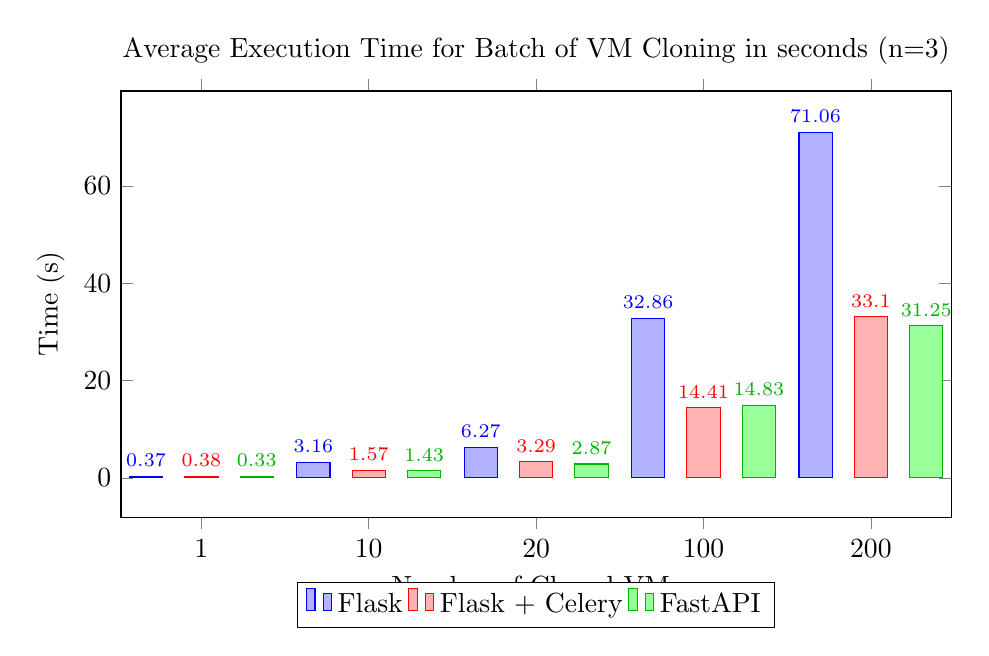
\begin{tikzpicture}
                    \begin{axis}[
                        title={Average Execution Time for Batch of VM Cloning in seconds (n=3)},
                        ybar,
                        bar width=12pt,
                        enlargelimits=0.12,
                        ylabel={Time (s)},
                        xlabel={Number of Cloned VMs},
                        symbolic x coords={1, 10, 20, 100, 200},
                        xtick=data,
                        legend style={at={(0.5,-0.15)}, anchor=north, legend columns=-1},
                        ylabel near ticks,
                        xlabel near ticks,
                        nodes near coords,
                        every node near coord/.append style={font=\scriptsize},
                        width=1\textwidth,
                        height=7cm,
                    ]

                    % Example dummy data: replace these values with your actual measurements

                    % Flask
                    \addplot+[style={blue, fill=blue!30}, bar shift=-20pt] plot coordinates {
                        (1, 0.368690)
                        (10, 3.163624)
                        (20, 6.265722)
                        (100, 32.864042)
                        (200, 71.062075)
                    };

                    % Flask + Celery
                    \addplot+[style={red, fill=red!30}, bar shift=0pt] plot coordinates {
                        (1, 0.377741)
                        (10, 1.565772)
                        (20, 3.287195)
                        (100, 14.412073)
                        (200, 33.095232)
                    };

                    % FastAPI
                    \addplot+[style={green!70!black, fill=green!40}, bar shift=20pt] plot coordinates {
                        (1, 0.330939)
                        (10, 1.434924)
                        (20, 2.872174)
                        (100, 14.832606)
                        (200, 31.253715)
                    };

                    \legend{Flask, Flask + Celery, FastAPI}
                    \end{axis}
                \end{tikzpicture}
                \caption{Average execution time to clone increasing number of\ac{vm}s across different implementations.}
                \label{fig:task2_plot}
            \end{figure}

            From Figure~\ref{fig:task2_plot}, we observe that the task completion time increases linearly with the number of 
            \ac{vm}s. The purely sequential Flask implementation consistently underperforms compared to the other two approaches, 
            except in the smallest batch size test, where no concurrency can be achieved.

            To compare the consistency of different implementations (Flask, Flask+Celery, FastAPI) across batch sizes, we first 
            normalize each run's execution time within its batch. For each combination of implementation and batch size, compute 
            the batch mean of the run times. Then calculate each run's percentage deviation from that mean using the standard 
            percent-change formula:

            \[
            \text{Deviation}_i = \frac{\text{time}_i - \text{batch\_mean}}{\text{batch\_mean}} \times 100\%.
            \]

            This normalization step effectively centers each batch's data at zero and removes scale differences. For example, 
            if a run is 10\,ms above a 100\,ms mean, its deviation is 
            \[
            \frac{10}{100} \times 100 = 10\%.
            \]
            This ensures that larger batch sizes, which naturally require more time, do not dominate the analysis. Instead, we 
            focus on the relative fluctuations around each batch's mean.

            \begin{figure}[ht]
                \centering
                \begin{tikzpicture}
                    \begin{axis}[
                            title={Execution Time Deviation for Batch VM Cloning (n=3)},
                            ylabel={Deviation (\%)},
                            boxplot/draw direction=y, % Vertical boxplot
                            xtick={1,2,3},
                            xticklabels={Flask,Flask + Celery,FastAPI},
                            width=1\textwidth,
                            height=6cm,
                        ]

                        % First dataset: Flask
                        \addplot+[boxplot] table[row sep=\\,y index=0] {
                         3.221134\\  0.112139\\ 1.133900\\
                        1.021761\\ 0.800631\\ 1.463433\\ 0.662802\\ 0.175874\\
                        0.020318\\ 0.196192\\ 0.151488\\ 0.440729\\ 0.592217\\
                        };

                        % Second dataset: Flask + Celery
                        \addplot+[boxplot] table[row sep=\\,y index=0] {
                        1.454436\\ 0.773281\\ 2.227717\\ 0.933618\\ 4.111049\\
                        3.177431\\ 5.191073\\ 1.166758\\
                        0.786188\\ 1.952946\\ 5.706726\\ 1.309611\\ 4.397116\\
                        };

                        % Third dataset: FastAPI
                        \addplot+[boxplot] table[row sep=\\,y index=0] {
                        0.493747\\ 3.698869\\ 3.205122\\ 1.216185\\ 0.476169\\
                        0.740016\\ 1.803419\\ 2.513543\\ 4.316962\\ 0.408508\\
                        0.784985\\ 0.376477\\ 0.903063\\ 2.445461\\ 1.542398\\
                        };

                    \end{axis}
                \end{tikzpicture}
                \caption{Boxplot comparison of execution time variability for VM cloning.}
                \label{fig:task2_boxplot}
            \end{figure}

            Once again, in Figure~\ref{fig:task2_boxplot}, we observe the same trend: the FastAPI implementation is slightly 
            faster and more consistent when compared to the Flask + Celery approach, altought the Flask sequential implementation 
            actually wins in this metric of deviation, being more consistent than the other two in run-to-run variation, at the cost of 
            being two times slower than the FastAPI implementation, making the FastAPI effort the overall better performer.


        \subsubsection{Task 3: VM Deletion}

            This task is much more short lived than the previous ones, consisting of a single\ac{api} call to\ac{pve} per\ac{vm} to 
            perform the deletion.

            Since the deletion operation does not require any preliminary validation or resource allocation, each\ac{vm} can be 
            removed independently without the need for coordination. This simplicity allows for rapid execution and straightforward 
            parallelization of the deletion process, with minimal overhead per\ac{vm}.
                        

            \begin{figure}[ht]
                \centering
                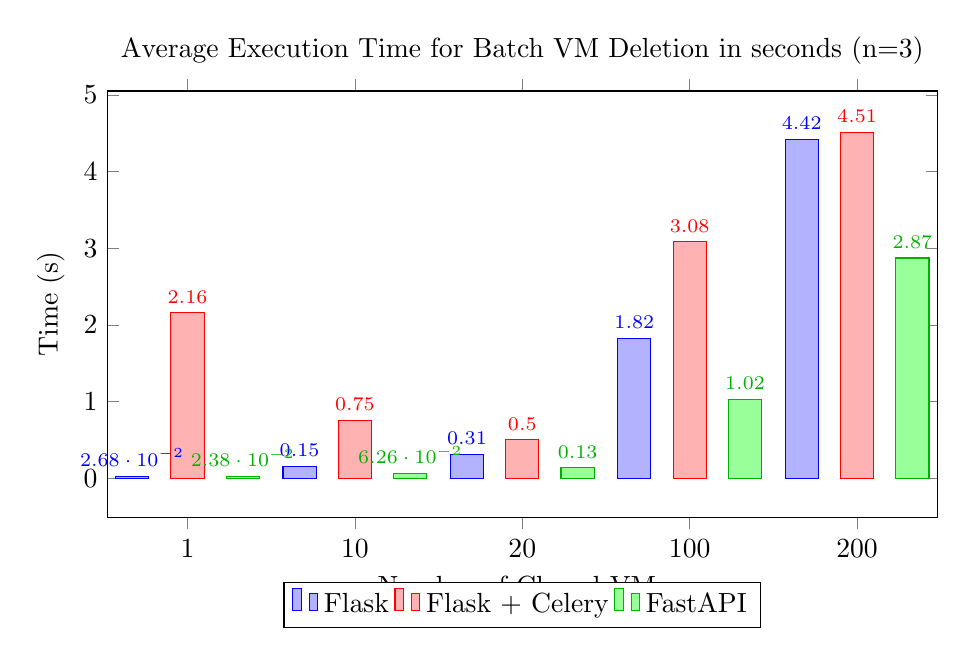
\begin{tikzpicture}
                    \begin{axis}[
                        title={Average Execution Time for Batch VM Deletion in seconds (n=3)},
                        ybar,
                        bar width=12pt,
                        enlargelimits=0.12,
                        ylabel={Time (s)},
                        xlabel={Number of Cloned VMs},
                        symbolic x coords={1, 10, 20, 100, 200},
                        xtick=data,
                        legend style={at={(0.5,-0.15)}, anchor=north, legend columns=-1},
                        ylabel near ticks,
                        xlabel near ticks,
                        nodes near coords,
                        every node near coord/.append style={font=\scriptsize},
                        width=1\textwidth,
                        height=7cm,
                    ]

                    % Flask
                    \addplot+[style={blue, fill=blue!30}, bar shift=-20pt] plot coordinates {
                        (1, 0.026849)
                        (10, 0.153751)
                        (20, 0.312510)
                        (100, 1.820313)
                        (200, 4.418675)
                    };

                    % Flask + Celery
                    \addplot+[style={red, fill=red!30}, bar shift=0pt] plot coordinates {
                        (1, 2.155812)
                        (10, 0.753148)
                        (20, 0.500132)
                        (100, 3.084107)
                        (200, 4.513475)
                    };

                    % FastAPI
                    \addplot+[style={green!70!black, fill=green!40}, bar shift=20pt] plot coordinates {
                        (1, 0.023758)
                        (10, 0.062618)
                        (20, 0.134784)
                        (100, 1.022950)
                        (200, 2.872160)
                    };

                    \legend{Flask, Flask + Celery, FastAPI}
                    \end{axis}
                \end{tikzpicture}
                \caption{Average execution time to delete increasing number of\ac{vm}s across different implementations.}
                \label{fig:task3_plot}
            \end{figure}

            In Figure~\ref{fig:task3_plot} we can see a textbook example of the overhead that Celery and the message broker 
            bring with them, and why it is not a good idea to use them for especially short-lived, non-\ac{cpu} intensive tasks. 
            The additional overhead introduced significantly impacts the overall execution time. 

            In this case, those two factors, the asynchronous orchestration and broker communication, have a higher influence on 
            execution time than the\ac{vm} batch size itself.

            In the particular case of sample size 1, we can see that it took even more time than bigger batch sizes. While this 
            may in part be fault of our relatively small data pool, we choose to keep it as it highlights very well the performance 
            overhead that celery brings with it, and why it can be considered detrimental in the case of short-lived tasks

            When comparing batch size 100 to 200, FastAPI exhibited a 2.8x slowdown despite only a 2x increase in workload. This disproportional 
            latency is not due to FastAPI itself, but rather to hitting performance limits in\ac{pve}. As infrastructure resources became saturated, 
            clone operations began failing and triggered exponential backoff retries, leading to higher cumulative delays.

            The other implementations scale in a much more expected manner, with the FastAPI version being 1.84x faster on average 
            than Flask.

            \begin{figure}[ht]
                \centering
                \begin{tikzpicture}
                    \begin{axis}[
                            title={Execution Time Deviation for Batch VM Deletion (n=3)},
                            ylabel={Deviation (\%)},
                            boxplot/draw direction=y, % Vertical boxplot
                            xtick={1,2,3},
                            xticklabels={Flask,Flask + Celery,FastAPI},
                            width=1\textwidth,
                            height=6cm,
                        ]

                        % First dataset: Flask
                        \addplot+[boxplot] table[row sep=\\,y index=0] {
                        1.466243\\ 0.254513\\ 1.211730\\ 1.705134\\ 0.029702\\ 
                        1.734836\\ 0.053972\\ 2.575067\\ 2.521095\\ 0.877047\\
                        0.594293\\ 1.471340\\ 0.669756\\ 0.299788\\ 0.369968\\
                        };

                        % Second dataset: Flask + Celery
                        \addplot+[boxplot] table[row sep=\\,y index=0] {
                        0.054210\\ 46.458512\\ 46.404302\\ 178.150500\\ 89.246465\\
                        88.904035\\ 69.954352\\ 135.324717\\ 65.370365\\ 64.345415\\
                        0.149854\\ 64.495269\\ 34.231252\\ 8.277547\\ 25.953705\\
                        };

                        % Third dataset: FastAPI
                        \addplot+[boxplot] table[row sep=\\,y index=0] {
                        1.491407\\ 2.526833\\ 4.018239\\ 0.849068\\ 6.666383\\
                        5.817315\\ 4.301698\\ 1.202665\\ 3.099033\\ 0.149600\\
                        0.913567\\ 1.063167\\ 0.735265\\ 0.763815\\ 0.028550\\
                        };

                    \end{axis}
                \end{tikzpicture}
                \caption{Boxplot comparison of execution time variability for VM deletion.}
                \label{fig:task3_boxplot}
            \end{figure}

            As shown in Figure~\ref{fig:task3_boxplot}, the Flask + Celery implementation exhibits significantly higher variability 
            during this task when compared to the other two approaches. The presence of numerous outliers and a wide interquartile range 
            highlight the inconsistency introduced by Celery and the message broker's overhead.

            \begin{figure}[ht]
                \centering
                \begin{tikzpicture}
                    \begin{axis}[
                            title={Execution Time Deviation for Batch VM Deletion (n=3)},
                            ylabel={Deviation (\%)},
                            boxplot/draw direction=y, % Vertical boxplot
                            xtick={1,2},
                            xticklabels={Flask,FastAPI},
                            width=1\textwidth,
                            height=6cm,
                        ]

                        % First dataset: Flask
                        \addplot+[boxplot] table[row sep=\\,y index=0] {
                        1.466243\\ 0.254513\\ 1.211730\\ 1.705134\\ 0.029702\\ 
                        1.734836\\ 0.053972\\ 2.575067\\ 2.521095\\ 0.877047\\
                        0.594293\\ 1.471340\\ 0.669756\\ 0.299788\\ 0.369968\\
                        };

                        % Third dataset: FastAPI
                        \addplot+[boxplot] table[row sep=\\,y index=0] {
                        1.491407\\ 2.526833\\ 4.018239\\ 0.849068\\ 6.666383\\
                        5.817315\\ 4.301698\\ 1.202665\\ 3.099033\\ 0.149600\\
                        0.913567\\ 1.063167\\ 0.735265\\ 0.763815\\ 0.028550\\
                        };

                    \end{axis}
                \end{tikzpicture}
                \caption{Boxplot comparison of execution time variability of Flask and FastAPI for VM deletion.}
                \label{fig:task3_boxplot2}
            \end{figure}

            Figure~\ref{fig:task3_boxplot2} isolates the Flask and FastAPI implementations for a clearer comparison. We observe that while 
            the Flask approach is slightly more consistent, as indicated by its tighter distribution.
        
    \subsection{I/O Problems during Batch VM Operations}
    \label{sec:io_problems}

        \begin{figure}[h]
        \centering
        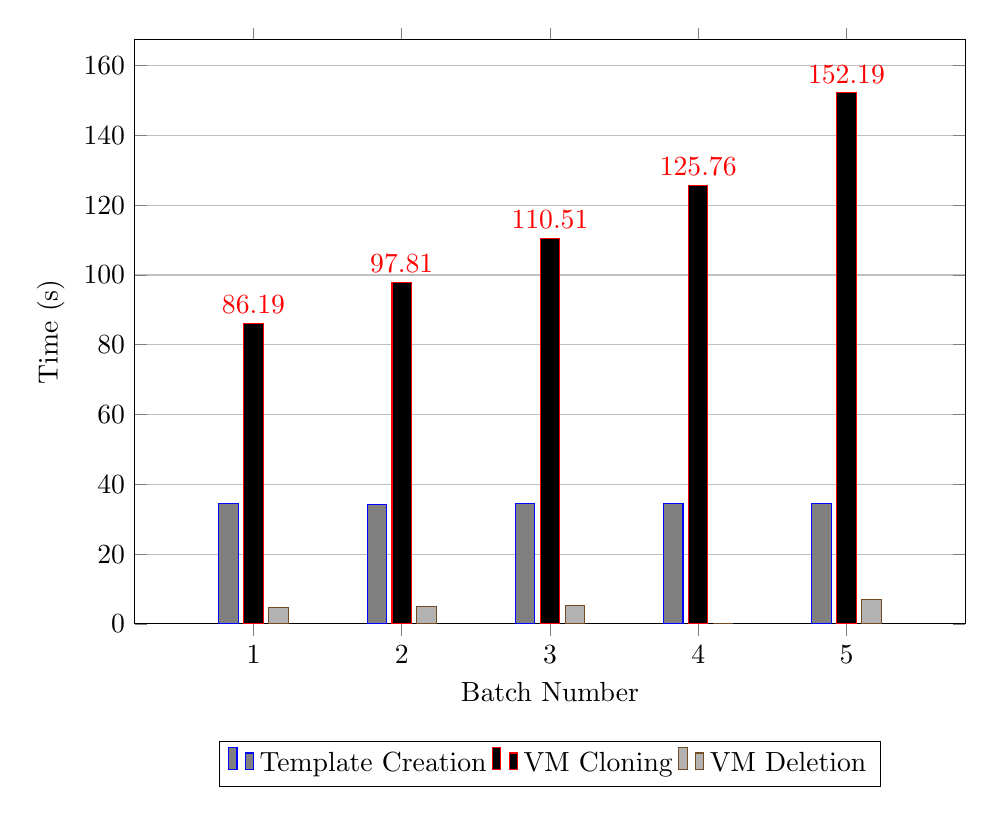
\begin{tikzpicture}
            \begin{axis}[
            ybar,
            bar width=7pt,
            width=\textwidth,
            height=9cm,
            ylabel={Time (s)},
            xlabel={Batch Number},
            symbolic x coords={1,2,3,4,5},
            xtick=data,
            ymin=0,
            enlarge x limits=0.2,
            legend style={at={(0.5,-0.2)}, anchor=north,legend columns=3},
            ymajorgrids=true,
            bar shift auto
            ]

                % Template creation (no labels)
                \addplot+[ybar, fill=gray] coordinates {
                (1,34.379) (2,34.312) (3,34.422) (4,34.609) (5,34.571)
                };
                \addlegendentry{Template Creation}

                % VM cloning (with labels)
                \addplot+[
                ybar,
                fill=black,
                nodes near coords,
                ] coordinates {
                (1,86.187) (2,97.805) (3,110.508) (4,125.758) (5,152.186)
                };
                \addlegendentry{VM Cloning}

                % VM deleting (no labels)
                \addplot+[ybar, fill=gray!60] coordinates {
                (1,4.612) (2,4.942) (3,5.377) (4,0.0) (5,7.090)
                };
                \addlegendentry{VM Deletion}

                \end{axis}
            \end{tikzpicture}
            \caption{Grouped bar chart showing VM operation times. Cloning time is labeled to highlight the rising trend. Results
            from Flask running purely sequential code}
            \label{fig:io_grouped_bar_plot}
        \end{figure}

        During initial stress tests of batch cloning and deletion of\ac{vm}s, 200 at a time, on our single node\ac{pve} cluster, 
        we observed rising task times in subsequent runs, specifically for the mass cloning of new\ac{vm}s, as can be seen in 
        Figure~\ref{fig:io_grouped_bar_plot}.

        It was also noted that there was an error thrown by\ac{pve} during the 4th batch of tasks, specifically during the 
        deleting task, causing it to fail.

        After some investigation it was found that there were intermittent failures to remove\ac{vm} disks. These failures 
        were \emph{not} detectable via the\ac{pve}\ac{http}\ac{api} responses and only appeared in the\ac{pve} server 
        logs. As orphaned disks accumulated, overall performance degraded significantly.
        \medskip

        \noindent\textbf{Observed Task History Outputs:}

\paragraph{1st type of output:} disk removed successfully

        \begin{verbatim}
trying to acquire lock...
OK
Logical volume "vm-348786940-disk-0" successfully removed.
TASK OK
        \end{verbatim}

\paragraph{2nd type of output:} intermittent lock-timeout failures followed by disk removed successfully

        \begin{verbatim}
trying to acquire lock...
Could not remove disk 'local-lvm:vm-120993831-disk-0', check manually:
can't lock file '/var/lock/pve-manager/pve-storage-local-lvm' - got timeout
trying to acquire lock...
OK
Logical volume "vm-120993831-disk-0" successfully removed.
TASK OK
        \end{verbatim}
        
\paragraph{ 3rd type of output:} failure to remove disk

        \begin{verbatim}
trying to acquire lock...
Could not remove disk 'local-lvm:vm-363495383-disk-0', check manually:
can't lock file '/var/lock/pve-manager/pve-storage-local-lvm' - got timeout
trying to acquire lock...
can't lock file '/var/lock/pve-manager/pve-storage-local-lvm' - got timeout
TASK OK
        \end{verbatim}

\paragraph{4th and final type of output:} storage config update errors and failure to remove disk

        \begin{verbatim}
trying to acquire lock...
Could not remove disk 'local-lvm:vm-5469324-disk-0', check manually:
can't lock file '/var/lock/pve-manager/pve-storage-local-lvm' - got timeout
trying to acquire lock...
can't lock file '/var/lock/pve-manager/pve-storage-local-lvm' - got timeout
trying to acquire cfs lock 'file-user_cfg' ...
TASK OK
        \end{verbatim}
                
        This suggests\ac{pve}'s locking mechanism can't keep pace with big amounts of deletion requests in quick succession.. 
        The lock is used to ensure that two tasks dont modify the\ac{lvm}'s metadata simulatenously. Since there should be 
        some underlying I/O tasks that are piling up, the system can't keep pace and eventually starts resorting to a retry mechanism 
        to keep up, but even this is insuficient and starts failing more and more towards the end as it becomes fully congested. 
        At the end, the system starts becoming overwhelmed and also begins having trouble updating its internal storage 
        config file.  

        This, combined with other factors were the main reason that led us to implement a hard limit on the amount of concurrent 
        requests that can be made from the web application to\ac{pve}\ac{api}. Still, while this significantly reduces the chances 
        of this problem reocurring, it does not fully remedy the problem and additional future work should look into solving this 
        matter completely.



        \begin{figure}[h]
        \centering
        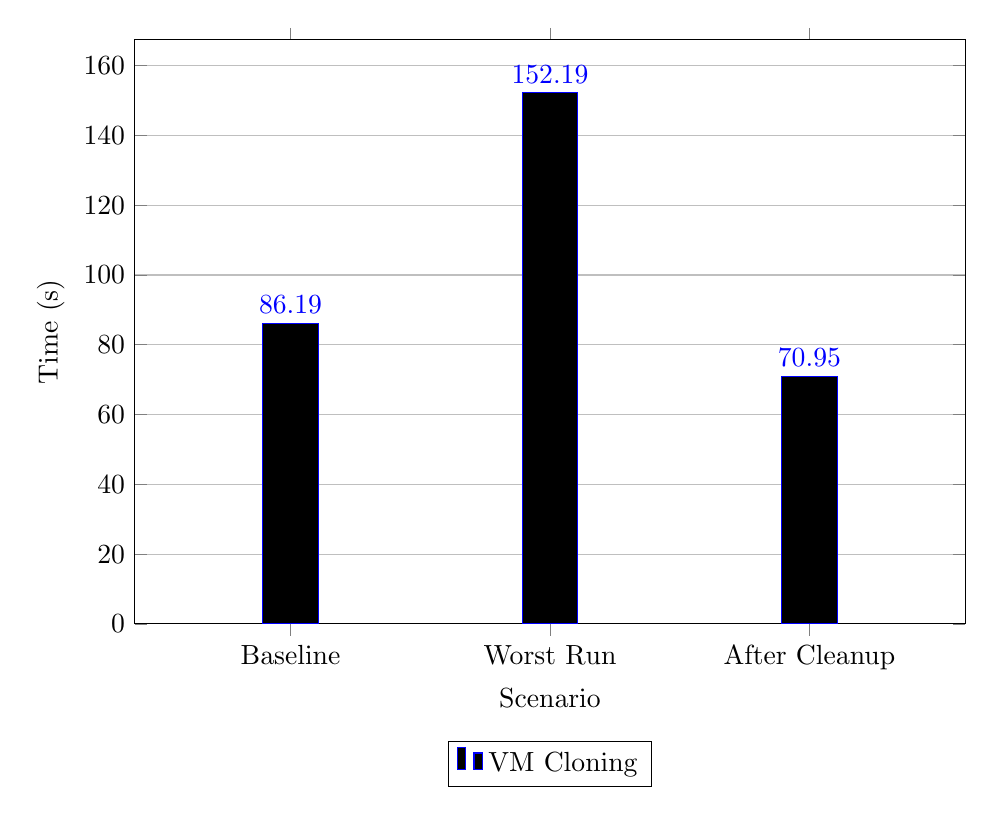
\begin{tikzpicture}
            \begin{axis}[
                ybar,
                bar width=20pt,
                width=\textwidth,
                height=9cm,
                ylabel={Time (s)},
                xlabel={Scenario},
                symbolic x coords={Baseline,Worst Run,After Cleanup},
                xtick=data,
                ymin=0,
                enlarge x limits=0.3,
                legend style={at={(0.5,-0.2)}, anchor=north, legend columns=1},
                ymajorgrids=true,
                nodes near coords
            ]

            % VM cloning bars without labels
            \addplot+[
                ybar,
                fill=black
            ] coordinates {
                (Baseline,86.187)
                (Worst Run,152.186)
                (After Cleanup,70.954)
            };
              
            \addlegendentry{VM Cloning}

            \end{axis}
        \end{tikzpicture}
        \caption{Bar chart showing VM cloning times after cleanup, at baseline, and in the worst case scenario.}
        \label{fig:vm_grouped_cloning_focus}
        \end{figure}

        After writing a small script to perform a cleanup of the orphaned disks we can see in 
        Figure~\ref{fig:vm_grouped_cloning_focus} that performance was improved from even our 1st recorded baseline test.

\section{System Usage}
    Due to the very early and prototipical\ac{ui} developed for the web application as well as lack of time to gather users in 
    order to perform usability tests, this section will contain a guide on how to perform various use cases.

    \subsection{Create a new exercise and enroll students}
        To start, the user must provide privileged credentials using the login form shown in Figure~\ref{fig:web_app_login}. 
        Without authorized credentials, the web application will not authorize the creation of new exercises.

        \begin{figure}
            \centering
            \includegraphics[width=5cm]{6TestingEvaluation/web_app_login.png}
            \caption{A screenshot of the login page}
            \label{fig:web_app_login}
        \end{figure}

        Next, the user should navigate to the ``Exercises" page via the navigation bar, and then select ``Create Exercise". This 
        will display the form shown in Figure~\ref{fig:web_app_create_exercise}.

        \begin{figure}
            \centering
            \includegraphics[width=10cm]{6TestingEvaluation/web_app_create_exercise.png}
            \caption{ A screenshot of the create exercise page}
            \label{fig:web_app_create_exercise}
        \end{figure}

        The form includes the following key fields:
        
        \begin{itemize}
             \item \textbf{Template VM Proxmox ID}:  This refers to the Proxmox ID of the template\ac{vm} to be cloned. 
             The template must meet the previously defined requirements: it should have\ac{gns3} installed and configured 
             to start automatically after boot, and it should contain the necessary network devices.
             \item \textbf{GNS3 Project File}: This field accepts a file with the \texttt{gns3project} extension, which can be exported 
             directly from\ac{gns3}.
             \item \textbf{Exercise validation}: This field allows the user to define one or more validation checks to be executed 
             on the specified devices. Currently, only \texttt{ping} and \texttt{traceroute} commands are supported. These validations will be executed 
             when a student requests automatic assessment.
             \item \textbf{Exercise pre-configuration}: This field enables the execution of custom commands on any supported device type 
             for initial configuration. These commands will be executed only on the template\ac{vm} before it is converted into a reusable 
             template.
        \end{itemize}

        After completing this process, clearing the functional use case described in Subsection~\ref{sec:new_exercise},the user should navigate to 
        the newly created exercises' page, as shown in Figure~\ref{fig:web_app_exercise}, and click on "Manage Exercise".

        \begin{figure}
            \centering
                \includegraphics[width=5cm]{6TestingEvaluation/web_app_exercise.png}
            \caption{ A screenshot of the exercise page}
            \label{fig:web_app_exercise}
        \end{figure}

        In the management interface (Figure~\ref{fig:web_app_manage_exercise}), the user can enroll or remove students from the exercise. Enrolling a 
        student automatically creates and assigns a dedicated\ac{vm}, completing the use case in Subsection~\ref{sec:enlist_users}, while removing them 
        destroys the corresponding\ac{vm}. It is important to note that exercises are only visible to students who are enrolled in them.

        \begin{figure}
            \centering
            \includegraphics[width=8cm]{6TestingEvaluation/web_app_manage_exercise.png}
            \caption{ A screenshot of the exercise management page}
            \label{fig:web_app_manage_exercise}
        \end{figure}

    \subsection{Complete an assignment and request an assessment}

        To begin, the user must log in using the form shown in Figure~\ref{fig:web_app_login}, ensuring the account is enrolled in at least one exercise. 
        After logging in, the user should navigate to the exercises page (Figure~\ref{fig:web_app_exercise}) and click on "Start Work Environment", described in
        Subsection~\ref{sec:starts_vm}.

        Once the environment has been initialized, the user can click on "Connect to Work Environment", which will redirect them to the gns3-web instance 
        hosted on their dedicated\ac{vm} for the selected exercise. Within the\ac{gns3} interface, the user should configure the available devices according 
        to the requirements specified in the exercise description.

        When ready, the user can click "Request Exercise Evaluation" to trigger the automated validation process, which checks whether the exercise has 
        been correctly configured.

        After the assessment is complete, the results are displayed on the page shown in Figure~\ref{fig:web_app_assessment_exercise}, as described in 
        Subsection~\ref{sec:submit_solution}.

        \begin{figure}
            \centering
            \includegraphics[width=10cm]{6TestingEvaluation/web_app_assessment_exercise.png}
            \caption{ A screenshot of the exercise management page}
            \label{fig:web_app_assessment_exercise}
        \end{figure}


% Write text in here
% Use \subsection and \subsubsection to organize text

% Chapter Template

% Main chapter title
%\chapter[toc version]{doc version}
\chapter{Conclusion \& Future Work}

% Short version of the title for the header
%\chaptermark{version for header}

% Chapter Label
% For referencing this chapter elsewhere, use \ref{ChapterTemplate}
\label{Chapter7ConclusionFutureWork}

This work explored the design and implementation of an automated network assessment system, building upon the work of 
\citet{santos2024}. The system was developed for the deployment and evaluation of networking assignments, with each 
student interacting with a dedicated\ac{gns3} environment hosted via\ac{pve}\ac{vm}s and with the intention of being used 
in both classroom and examination settings, allowing instructors to allocate more time toward guiding and supporting 
students, rather than spending it on manual evaluation.

Throughout the project, several key aims and objectives were successfully met. A modular architecture was established, 
enabling the creation, management, and evaluation of network assignments. Integration with\ac{pve} allowed for 
automated\ac{vm} lifecycle management, while\ac{gns3} provided a flexible environment for deploying practical networking 
scenarios. With assessment being done with Nornir, which enabled scalable and repeatable command execution across multiple 
devices, and a web back-end built using FastAPI that facilitated communication between all system components.

One of the central objectives was to allow students to initiate assessments on demand. This was achieved through the use of 
the developed modules, which input a command to a given virtual network device, determine the correct command depending of 
its type (e.g. Cisco router, Linux VM have different syntax for a \texttt{traceroute}). This effort was made to ensure support for a 
diverse range of device types and vendors, as exposure to heterogeneous network environments better prepares students for 
the complexity of professional settings. While the current implementations has only support for a few device types, the 
modular structure can easily be expanded upon for broader compatibility in the future. The modules developed during the 
project offer a basis for extensibility.

Another major aim of this project was also to unify and extend the components originally developed by \citet{santos2024} into 
a cohesive back-end system. This required significant development effort, particularly in defining clear interfaces between 
components and ensuring they could operate together reliably under various conditions.

Significant progress was also made in terms of asynchronous handling and\ac{api} development. The\ac{api} design was 
iteratively refined to ensure clear boundaries between responsibilities while maintaining ease of integration with other 
components.


\section{Lessons learned}
    This project highlighted several important lessons, one of them being the criticality of asynchronous I/O in system 
    involving remote\ac{api} calls. For this, Python's asynchronous capabilities, in conjunction with libraries that support 
    them, proved invaluable. Additionally, it taught us key lessons in\ac{api} design, particularly that modularity facilitates 
    maintainability and integration, especially when multiple external systems are involved (\ac{pve},\ac{gns3}). 

    Additionally, we learned that error handling, observability, and retry mechanisms should be devised and implemented from the 
    the very early steps of development in networked systems, where silent failures during provisioning can propagate and lead to 
    complex, hard-to-diagnose issues.

    One more important lesson is the need to run tests periodically to ensure good system performance, as we found during 
    our tests that our performance was decreasing with no major errors to be seen anywhere, which highlights the importance of 
    monitoring and benchmarking.


\section{Future Work}
    Building on the current system, future work should aim for several things. In terms of security and access control, the 
    groundwork was laid for role-based authentication. However, further exploration is needed into\ac{pve}'s native role and 
    permission system. At present, \ac{pve} grants full administrative access to authenticated users, which is acceptable for development environments 
    but poses significant security concerns in production. Currently, role-based access control is enforced solely within the web 
    application layer, meaning that users such as students and teachers interact with the underlying\ac{pve} infrastructure using elevated 
    privileges. A more secure and fine-grained authorization model—where roles like "student" and "teacher" are mapped to 
    corresponding restricted scopes within\ac{pve} itself—remains a critical area for future development. Implementing this would 
    help enforce the principle of least privilege and provide a more robust separation of concerns between the application logic and 
    infrastructure permissions.

    It would also be desirable to expand on the assignment definition model to introduce versioning, as well as introducing 
    capabilities to create more complex grading of exercises including but not limited to adding exercise sub-lines and 
    support for boolean expressions in lines and sublines. 

    Additionally improving on the\ac{ui} using more modern frontend frameworks and shifting to Client Side Rendering could allow 
    for a better UX with new features such as real time feedback and progress tracking of interactions with services external 
    to the web application.

    Developing more, but also introducing more complex modules, capable of chaining commands, and supporting a much wider range 
    of devices is key in making sure this system can go overcome the limitations of its existing counterparts, such as Cisco's 
    Packet Tracer, by supporting more complex, multi-step, assessment of protocols and configurations not available to them.

    Furthermore, exploring the capabilities and limitations of the system in a multi-node cluster environment presents a 
    another direction for future work. While\ac{pve} offers robust support for clustering and centralized management of multiple 
    nodes, it does not natively include mechanisms for automated load balancing across those nodes. In the current implementation,\ac{vm} 
    placement decisions must be made manually, which can lead to inefficient resource utilization, especially under dynamic 
    or heavy workloads. Developing an integrated load balancing feature could significantly enhance scalability, fault tolerance, 
    and system responsiveness. This would involve monitoring node resource usage in real-time and dynamically provisioning or migrating 
    ac{vm}s to balance\ac{cpu} and memory loads more effectively across the cluster.

    Another promising direction for future work lies in providing optional containerized environments for student exercises. While 
    this was not pursued in the current implementation due to the lack of time to perform a thorough risk analysis, the potential 
    benefits justify further investigation. Containerization could reduce resource usage and startup times for exercises that do 
    not require full virtualization, such as those relying solely on\ac{iou} and\ac{vpcs} as well as others that do not rely on\ac{kvm}. 
    
    Simultaneously, as the system grows, it will be vital to integrate unit and system tests to ensure reliability and 
    maintainability as the platform scales, to ensure the continued good functioning of older parts.

    In conclusion, this system represents a promising step toward a fully automated and scalable platform for practical 
    networking education. While there is still much work to be done before it can be fully integrated in institutions and courses, 
    the progress made so far provides a strong basis for further growth and refinement.


% Write text in here
% Use \subsection and \subsubsection to organize text



% Add others as needed


%-------------------------------------------------------------------------
%	BIBLIOGRAPHY
%-------------------------------------------------------------------------
\addvspacetoc{0.5cm}
\addtotoc{Bibliography}

%\fancyhead[LO]{\textsc{Bibliography}}

 % The references are stored in the file "Bibliography.bib"
\bibliography{Bibliography}

%-------------------------------------------------------------------------
%	THESIS CONTENT - APPENDICES
%-------------------------------------------------------------------------

\appendix % Cue to tell LaTeX that the following 'chapters' are Appendices

%%% -----------  ADD APPENDIX HERE ------------------ %%%

%\input{Appendices/AppendixTemplate}
% Appendix Template

\chapter*{nornir\_lib documentation} % Main appendix title

\label{nornir_lib_appendix} % Change X to a consecutive letter; for referencing this appendix elsewhere, use \ref{AppendixX}

This library is responsible for connecting to\ac{gns3} devices in a given topology, inputting commands, retrieving output, and analyzing results to evaluate success or failure.

It consists of the following components:

\begin{itemize}
  \item \textbf{\texttt{modules/}} – Described in detail in the Subsection~\ref{sec:new_module}. Contains predefined command modules.
  \item \textbf{\texttt{utils/}} – Provides helper functions that interface with\ac{gns3} or facilitate command execution.
\end{itemize}

Additionally, it uses several configuration files located in the \texttt{app/} folder:

\begin{itemize}
  \item \texttt{config.yaml}  
  Contains paths to the \texttt{host\_file}, \texttt{group\_file}, and \texttt{defaults\_file}, as well as the configuration of the Nornir \texttt{runner}.
  
  \item \texttt{host\_file}  
  Describes the VMs or containers hosting\ac{gns3} servers. At minimum, the IP address, group (typically \texttt{linux}), username, and password (in plain text) must be specified.

  \item \texttt{group\_file}  
  Defines default settings for groups. \textbf{Note:} \texttt{fast\_cli} must remain \texttt{false} to ensure tests run reliably.

  \item \texttt{defaults\_file}  
  Currently unused.
\end{itemize}

\subsection*{Modules}

The project comes with built-in test modules. To use a module:

\begin{enumerate}
  \item Instantiate the module class by passing the configured Nornir object for the desired machine/project.
  \item Call the \texttt{command()} method with the required arguments, which may vary by module.
\end{enumerate}

\subsection*{Implementing a New Module}
\label{sec:new_module}

To create a custom module:

\begin{itemize}
  \item Subclass the \texttt{CommandModule} class located in \texttt{modules/module.py}.
  \item Implement the following methods:
    \begin{itemize}
      \item \texttt{\_command\_router}
      \item \texttt{\_command\_switch}
      \item \texttt{\_command\_vpcs}
      \item \texttt{\_command\_linux}
      \item \texttt{interpret\_cisco\_response}
      \item \texttt{interpret\_linux\_response}
      \item \texttt{interpret\_vpcs\_response}
    \end{itemize}
  \item For command methods, use \texttt{PingModule} as a skeleton and modify the command string accordingly.
  \item For interpretation methods, implement logic that evaluates command output and determines whether it meets expected results.
\end{itemize}


\chapter*{proxmox\_api endpoints} % Main appendix title

\label{pve_api_appendix} % Change X to a consecutive letter; for referencing this appendix elsewhere, use \ref{AppendixX}

This library is responsible for interacting with the Proxmox VE API, automating management tasks such as starting, stopping, and templating virtual machines and containers.  

Unless otherwise specified, all methods return a boolean value. In the event of network errors:
\begin{itemize}
  \item Functions expecting a boolean will return \texttt{False}.
  \item Functions expecting other types will return \texttt{None}.
\end{itemize}

All other exceptions are propagated and should be caught by the caller.

\subsection*{Module: \texttt{proxmox\_vm\_actions}}

\begin{verbatim}
_get_status(proxmox_host, session, vm_id)
    Queries the state of a VM. For internal use. Returns the raw response.

acheck_free_id(proxmox_host, session, id)
    Checks if given VM/CT ID is unused. Does not reserve it.

create(proxmox_host, session, template_id, clone_id, hostnames)
    Clones the specified template VM with the given hostname.

check_vm_status(proxmox_host, session, vm_id)
    Checks if the VM is running and the QEMU guest-agent is active.

check_vm_is_template(proxmox_host, session, vm_id)
    Checks if a VM is in template format.

start(proxmox_host, session, vm_id)
    Starts the specified VM.

stop(proxmox_host, session, vm_id)
    Stops the specified VM.

template(proxmox_host, session, vm_id)
    Transforms the VM into a template.

destroy(proxmox_host, session, vm_id)
    Destroys the specified VM.
\end{verbatim}

The \texttt{session} parameter must be created using the \texttt{connection} module in \texttt{utils/}, and must contain valid credentials for the Proxmox cluster.

\subsection*{Module: \texttt{proxmox\_vm\_firewall}}

\begin{verbatim}
create_proxmox_vm_isolation_rules(proxmox_host, first_vm_id, last_vm_id, allowed_vm_ip, session)
    Enables firewall and blocks communication between student VMs.
    Only allows communication with the allowed VM (typically the teacher VM).

delete_proxmox_vm_isolation_rules(proxmox_host, first_vm_id, last_vm_id, allowed_vm_ip, session)
    Removes previously set firewall rules, re-enabling inter-VM communication.
\end{verbatim}

\subsection*{Module: \texttt{utils}}

Various utility functions to support Proxmox interaction:
\begin{itemize}
  \item \texttt{connection.proxmox\_connect}:  
    Authenticates and returns an HTTP session with a valid authentication cookie.  
    See the ProxmoxVE authentication documentation for details.
    
  \item \texttt{proxmox\_base\_uri\_generator}:  
    Generates the base URI for API calls to Proxmox.

  \item \texttt{proxmox\_vm\_ip\_fetcher}:  
    Retrieves the current IP address or hostname of a VM or container given its ID.
\end{itemize}

\backmatter


\end{document}
